\documentclass[a4paper,12pt,UTF8]{article}
\usepackage[notoc,noabs]{HaotianReport}

\title{基于文本数据挖掘的官媒主题效力分析}
\author{刘昊天}
\authorinfo{lht18@mails.tsinghua.edu.cn}
\runninghead{清华大学《政务大数据》2019秋季学期}
\studytime{2019年12月}
\graphicspath{{./}{./img/}{./fig/}{./image/}{./figure/}{./picture/}{./pic/}}
\begin{document}
    \maketitle
    \section{研究背景}
    所谓“官媒”,通常指的是有政府背景,由政府部门创办的媒体。它具有专用、权威、公开等性质,是官方监督与纠正不良现象、协调社会关系、传承文化、提供娱乐、引导大众、传播资讯的重要渠道\cite{guanmei}。一直以来,官媒都有其独有的优势,包括公信力优势、资金政策优势、人才优势和融媒体优势\cite{李志明2017区域性官媒和自媒体微信公众号差异化分析}。如何更好地发挥官媒优势,增强官媒的影响力与传播力,进而更充分地完成官方赋予官媒的使命,是官方机构工作人员长期以来关注的问题。

    传统的官媒形式包括报纸、电台、电视等,在新中国建设中发挥过重要作用。然而,随着网络时代的到来,智能手机不断普及,移动社交软件已经渐渐成为人们生活的重要组成部分,媒介形式也迎来了翻天覆地的变化。最有代表性的微信,作为目前腾讯旗下赶超 QQ 的社交软件,更是在前几年迎来爆发式增长。根据腾讯控股 [00700]2018年年报,截止至 2018 年 12 月 31,微信合并月活跃用户数达 10.98 亿,同比增长 11.0\%;同时, 2018 年腾讯的网络广告业务收入达 581 亿元,同比增长 44\%。

    在微信及腾讯广告业务的发展过程中,微信公众号功不可没,其已经成为了国内最大的内容提供平台之一,也从一种社交新宠逐渐演变成民间自媒体的一种主要形式并几近泛滥。个人或企业用户可以在微信公众号上发布文章,通过微信的订阅服务定向推送给已订阅的用户,无论是宣传还是营收都有巨大的空间;已订阅用户则可以消费微信公众号的推送内容。数据显示,2013年至2017年,微信公众号数量增长近10倍,如\cref{fig:pub}所示。
    由此可见,微信公众号已经并将在很长一段时间内继续扮演中国人生活中的重要角色。

    \begin{figure}
      \centering
      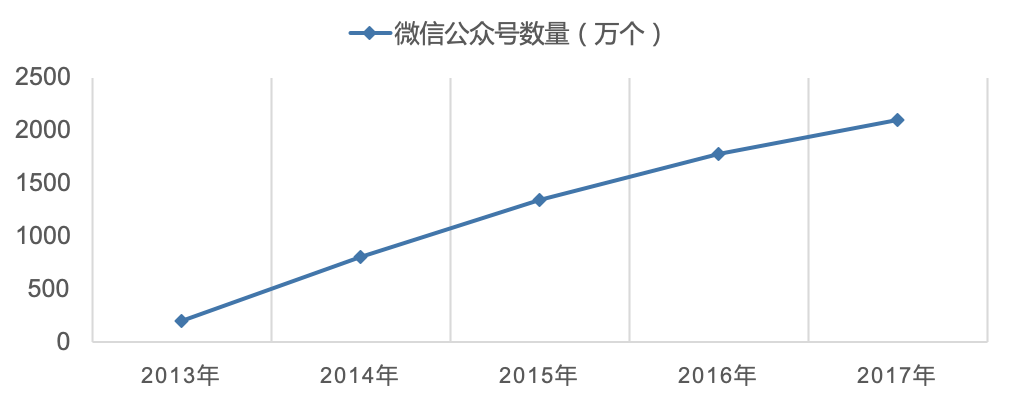
\includegraphics[width=0.9\linewidth]{pub.png}
      \caption{微信公众号数量统计}
      \label{fig:pub}
    \end{figure}

    为顺应该形势,近年来各地政府纷纷开通微信公众号作为官媒的新形式,发挥着宣传渠道、服务平台与展示窗口的关键作用。由此,本文拟采用官方或官方媒体的微信公众号作为官媒的代表进行研究。

    \section{研究问题}
    尽管官媒发布的内容往往是经由工作团队精心挑选或编写的,但受众并非对于官媒发布的所有内容都感到兴趣。换言之,即便在相同的官媒中,发布不同的官媒内容也将呈现出不同的传播效力。

    以目前微信平台上目前最大的官方媒体之一“人民日报”为例,2019年8月19日发布的题为《为了一名高三女孩,末班公交每天多等5分钟,直到她考上大学……》一文,收获了10万以上阅读量,10万以上点赞量;而在2019年8月26日发布的题为《【提醒】微信工作群“说错话”,被公司状告赔偿46万》一文,尽管同样收获了10万以上阅读量,却只有767点赞量。
    
    再以吉林省的官方媒体之一“吉林日报”为例,其平均阅读量和点赞量都远不及“人民日报”。2019年10月9日发布的题为《定了!吉林省这些院校和专业成为省级示范,有你的母校吗?》一文,收获了90906阅读量和302点赞量;而在2019年11月15日发布的题为《动车票低至6.5折、敞开办理团体票业务…吉林车务段推出超多优惠!》一文,却仅收获了670阅读量和3点赞量。
    
    由此两例可见,官媒发布的文本内容同传播效力之间存在一定的联系。本文的目标即为刻画官媒文本内容同该内容传播效力之间的关系(简称“内容-效力关系”),为官媒内容发布提供参考。特别地,选取文本内容的主题作为核心特征,因其一方面易于被人们解读,另一方面也能将文本数据转换为数值数据,便于分析。本文的到的相关结构,可以指导官媒在媒介资源有限的条件下最大化传播效力,充分发挥官媒功能。

    另外,本文也希望通过对比官媒与非官媒、不同官媒之间的内容-效力关系,分析各个公众号的内容特质。

    在调研中发现,目前微信平台上的官媒主要分为两种,一种是由政府直接运营的“政府发布”类公众号,名称均为“XX(城市)发布”。因有关政策的限制,这一类公众号无法由第三方机构注册,因此具有较高的权威性。另一种是在政府控制下的媒体,例如前文提到的“人民日报”和“吉林日报”,我们即称之为“官方媒体”。其他非官媒的公众号,主要是有“机构媒体”和“内容运营”两类。前者不以盈利为目的,主要发挥宣传、服务等功能性作用。后者目标为通过内容盈利,往往发布较多的原创内容。
    \section{研究方法}
    \subsection{主题提取}
    在对大量的公众号文章进行文本挖掘时, 一个自然的想法是利用一系列可以概括文章内容的主题来对文本库进行分析归纳。本文采用的主题模型一方面将大量繁杂的文章映射到一组低维度主题词上,另一方面,不同于简单的文本聚类模型,聚类后每篇文章仅能属于一个主题类别,主题模型可以在对文章进行分类整合的同时,允许不同文章间内容和立意的重叠,并能量化地表现出主题的相似度。

    在实际进行主题提取时, 本文采用文本挖掘领域最常用且有效的主题模型算法LDA(Latent Dirichlet Allocation), 这一算法基于对文本建立主题模型过程中所遵循的两个核心原则:
    
    \begin{itemize}
      \item \textbf{每篇文章是一系列主题的组合}:每篇文章包含了以一定比例混合的主题。比如, 文档一包含$10\%$的A主题和$90\%$的B主题; 文档二包含了$80\%$的A主题和$20\%$的B主题;
      \item \textbf{每个主题是一系列词语的组合}:主题的产生源于以一定比例混合的词语。比如
      娱乐主题中包含“电影”“电视”等词;政治主题中则更多包含“环境”、“民生”等词。值得注意的是,每个主题下所包含的关键词及其配比并非通过先验知识人为给定,而是在整个大的文本数据库中,利用无监督的机器学习算法提取而出。
    \end{itemize}
    
    \subsection{多元回归分析}
    多元回归分析主要用于分析响应变量与一系列解释变量之间的线性相关性和依赖性,以此来进行统计解释、推断和预测。记$Y$为我们所关心的响应变量,$V_1,...,V_K$为解释变量,回归分析所基于的多元线性模型为:
    \begin{equation}\label{lm}
      Y = \beta_0+ \beta_1 V_1+...+\beta_K V_K +\epsilon,
    \end{equation}
    这里$\epsilon \sim N(0,\sigma^2)$ 为模型中引入的同方差独立高斯噪声。
    
    利用最小二乘法,我们可以得到对线性模型参数的估计量$\hat\beta_0,...,\hat\beta_K$以及其他相关回归统计量。根据模型(\ref{lm}),我们可以进行以下统计推断:
    \begin{itemize}
      \item 回归得到的改进的$R^2$系数和$F$统计量对应的p值可以用来衡量线性模型整体的显著性;
      \item 每个解释变量系数所对应的t统计量及其对应的p值可用于衡量该单一变量在模型中的显著性;
      \item 当解释变量线性无关且具有相同量纲时,多元回归得到的变量系数大小可以用来比较解释变量对响应变量的影响大小;而变量系数的符号则可用来衡量该解释变量对响应变量(文章效力)的作用方向。
    \end{itemize}

    多元线性回归的模型假设中,要求模型(\ref{lm})中$\epsilon$ 服从正态分布,故而响应变量$Y$即本文所研究的微信文章的效力数据也应服从正态分布。所以在建模前,为验证模型的可行性,我们对数据进行了分布检验,如图中的qq图所示,数据点在qq图上的排布近似线性,即数据满足正态性假设,故而本文建立的多元回归模型是合理的。

    \section{数据来源及变量测量}
    \subsection{数据来源}
    本文所涉及到的数据,均为微信公众号数据,通过爬虫的方式从公开访问渠道获取。数据平台采用了本人上个学期开发的一套微信公众号数据可视化系统(\url{https://github.com/ritou11/wxPubVis}),实现了从数据获取到简单的数据展示全过程。爬取数据的基本过程为:
    \begin{enumerate}
      \item 确定待研究公众号及时间范围。由于爬取数据的方式是逐个公众号、逐篇推送地从微信获取,爬取速度有限,因此必须确定一个需要获取推送数据的范围,包括公众号范围和时间范围\thanks{部分公众号为王健骁同学推荐}。在本文中,公众号主要选取政府发布和官方媒体两类,另外包含少量的机构媒体和内容运营类公众号。时间上选择为2018年1月1日至2019年11月1日,即近两年时间。
      \item 准备微信账号。登陆作为爬虫的微信账号并关注待爬取的公众号。
      \item 接入平台并信任证书。在本人开发的微信公众号数据可视化系统中,采用了“中间人”的方式爬取微信公众号数据,即在网络层面劫持微信数据包,读取其中的内容并实现在线跳转。这部分采用的核心代码从开源项目wechat\_spider(\url{https://github.com/lqqyt2423/wechat_spider})改编而来。
      \item 触发推送并开始自动爬取。手动在微信客户端上访问公众号的信息页面,即可将其标记为待爬取公众号。全部标记完成后,访问任一待爬取公众号的信息页面即可触发推送列表的自动爬取。当全部列表爬取完成后,访问任意一篇推送即可开始爬取推送原文。
      \item 查看可视化内容并获取数据。数据储存在MongoDB数据库中,可导出为json文件或直接拷贝数据库。爬取的公众号信息包括:名称、头像、更新时间、标识码。爬取的推送信息包括:名称、封面、公众号、发布时间、评论(含点赞数)、内容(纯文本)、点赞数、阅读量。
    \end{enumerate}
    \subsection{样本描述}
    通过上述的数据获取方式,共获取到官媒相关公众号19项,非官媒公众号20项。各公众号在给定时间范围内的推送总数如\cref{fig:profiles}所示。其中,WPI为该公众号的传播力度量,将在\cref{sub:xiaoli}中提及,数值越大代表传播力越高。
    \begin{figure}
      \centering
      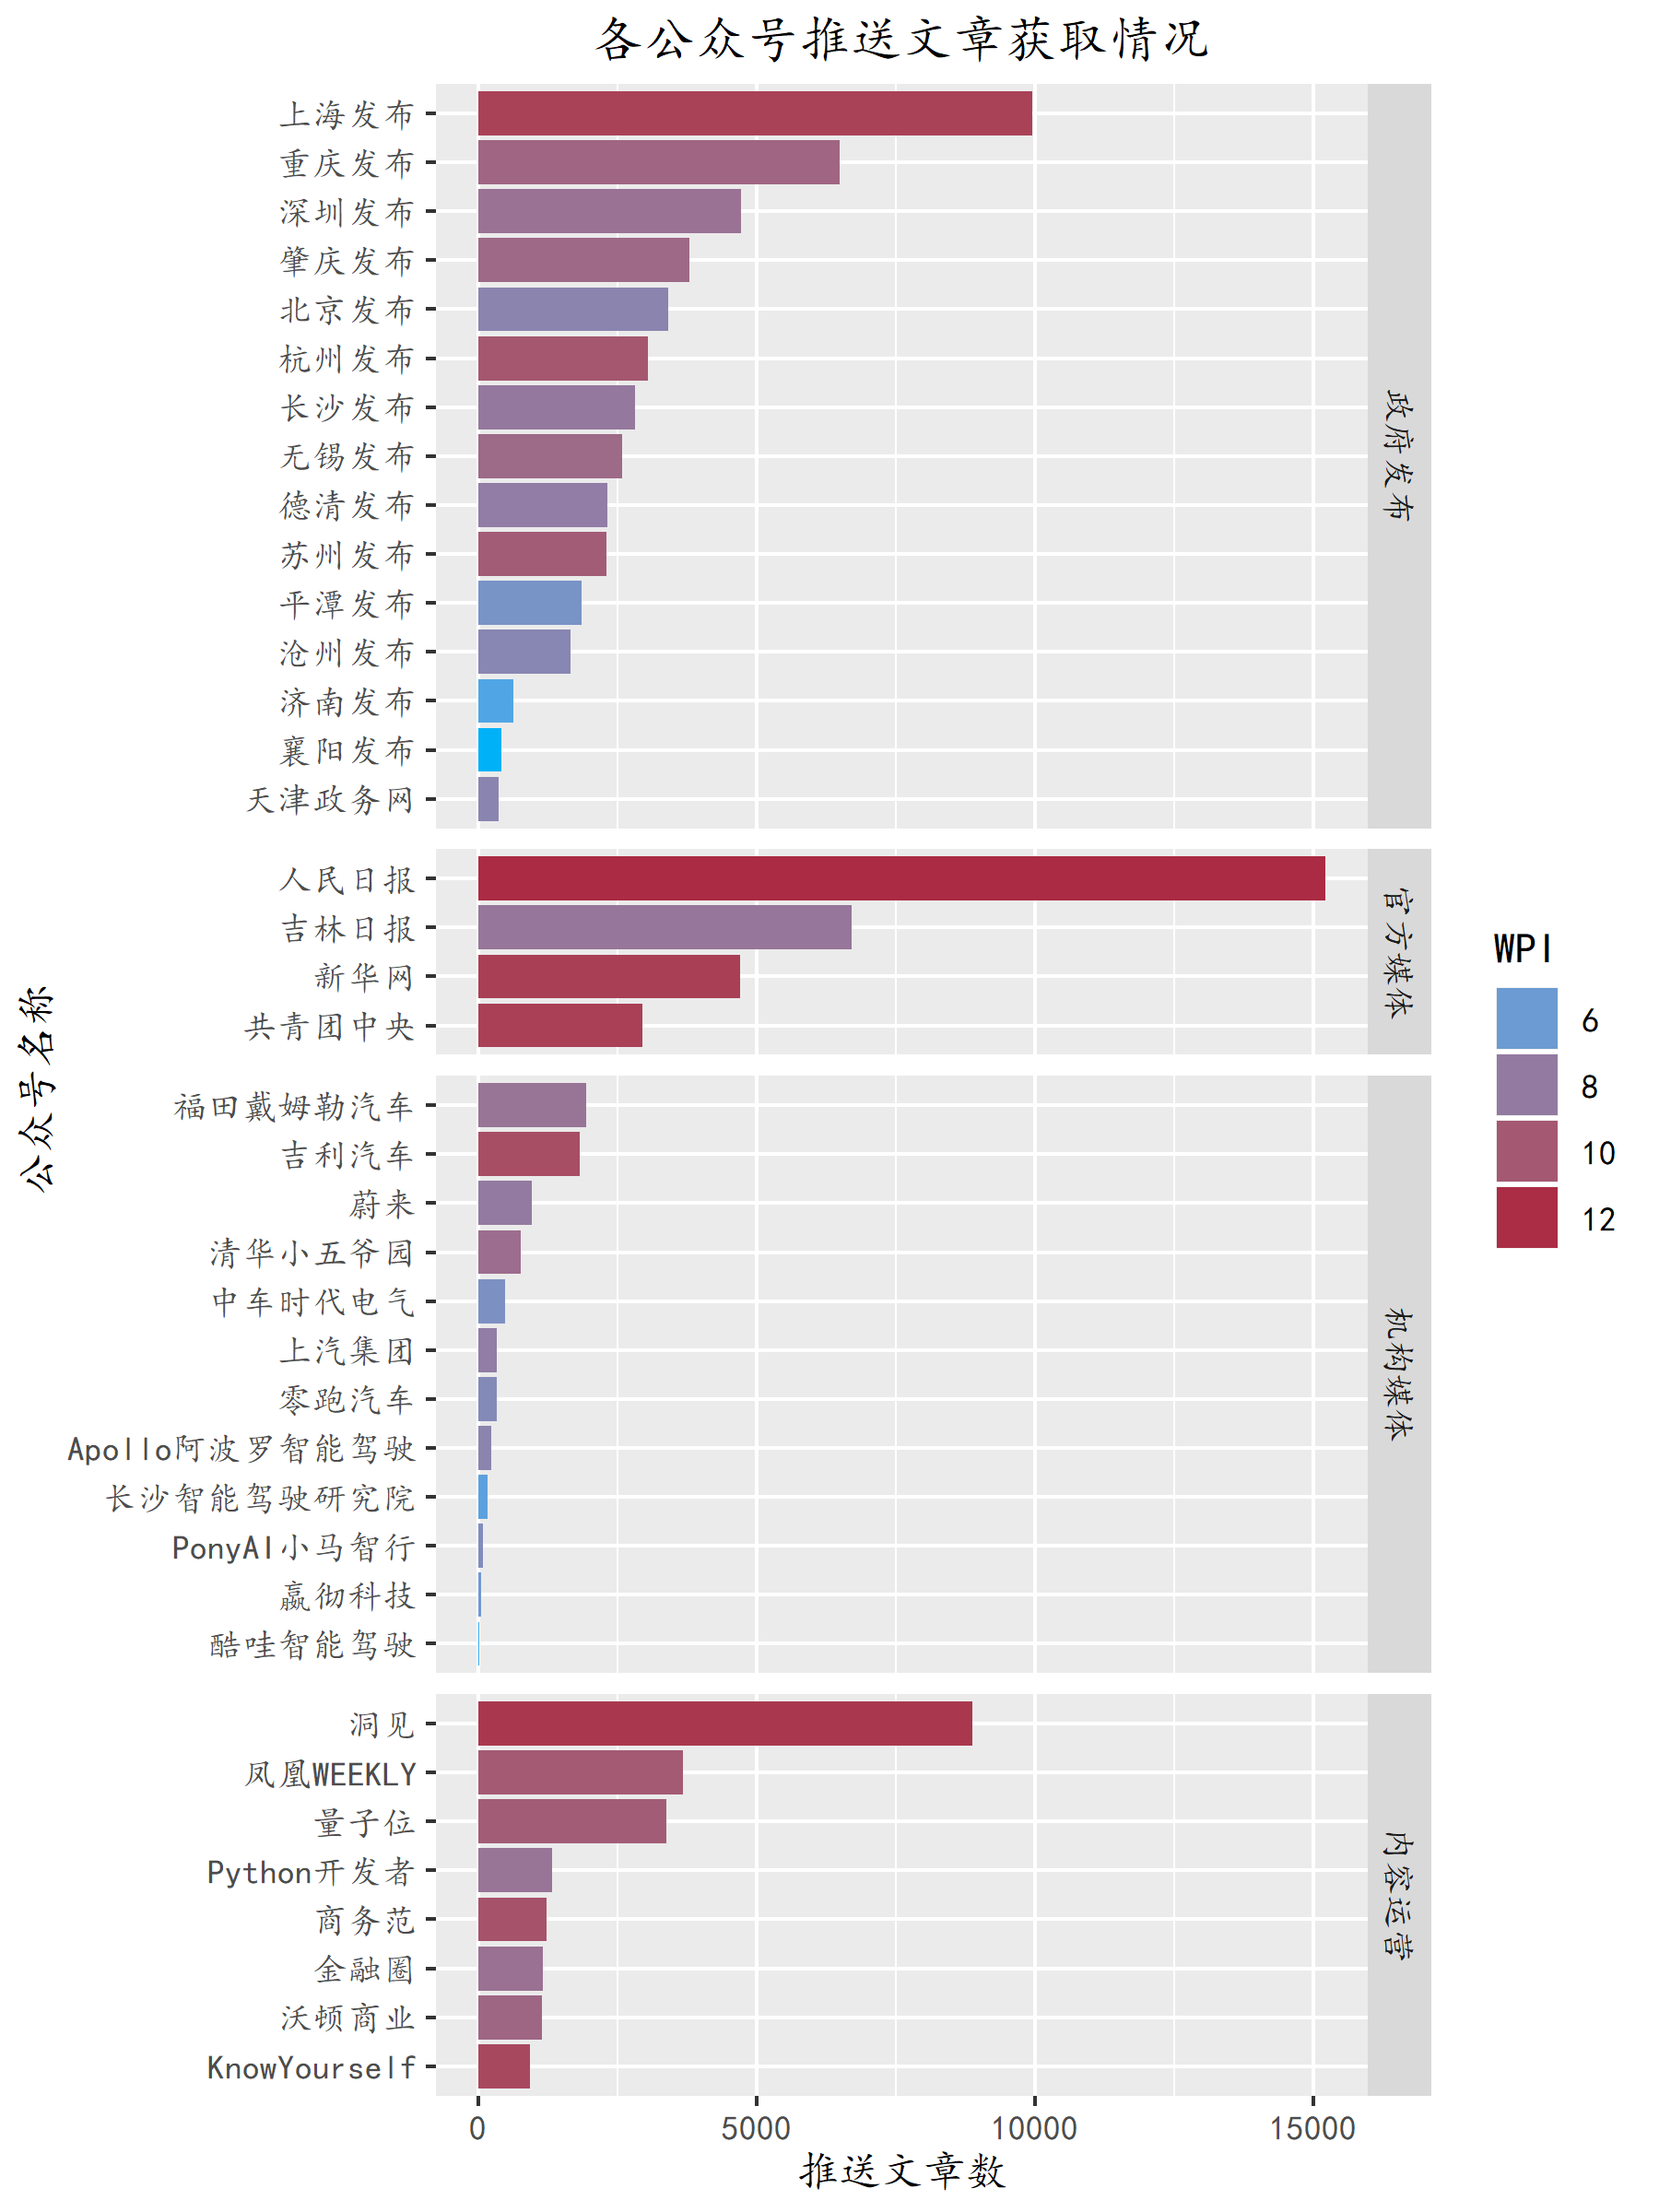
\includegraphics[width=0.9\linewidth]{profiles.png}
      \caption{公众号数据获取情况}
      \label{fig:profiles}
    \end{figure}
    
    从图中可见,官媒公众号的发布数量,要远大于非官媒公众号数量。事实上,根据本人的观察,官媒公众号可以每天多次发布信息,其单日发送的推送上限要远高于普通的机构媒体和内容运营公众号。另外,上海、重庆、深圳的政府发布公众号在所有观测公众号中累计发布数量位列前三,人民日报公众号在所有观测公众号中累计发布数量遥遥领先,传播力也同样很高。这一类排名靠前的公众号,因其运营更好、数据更多,更具备分析的价值。
    \subsection{效力分析}
    \label{sub:xiaoli}
    在本文中,对推送效力、公众号效力的量化分析是至关重要的。所谓效力的量化分析,即是建立从推文或公众号数据,到效力量化指标的映射。
    
    清博大数据对于该问题提出了一种名为微信传播指数WCI的公众号传播效力分析方法\cite{清博大数据2020}。分别记总阅读数$R$,总在看(点赞)数$Z$,最大阅读数$R_{max}$,最大在看数$Z_{max}$,头条总阅读数$R_t$,头条总在看数$Z_t$,统计总天数$d$,统计总篇数$n$。则WCI指数计算方式如\cref{eq:wci}所示。
    \begin{equation}
      \label{eq:wci}
      \begin{aligned}
        \text{WCI} &= \left\{ 0.3\left[0.85 \ln (\frac{R}{d} + 1)+ 0.15 \ln (\frac{10Z}{d} + 1)\right] \right. \\
                   &+ 0.3\left[0.85 \ln (\frac{R}{n} + 1)+ 0.15 \ln (\frac{10Z}{n} + 1)\right] \\
                   &+ 0.1\left[0.85 \ln (R_{max} + 1)+ 0.15 \ln (10Z_{max} + 1)\right] \\
                   &\left. + 0.3\left[0.85 \ln (\frac{R_t}{d} + 1)+ 0.15 \ln (\frac{10Z_t}{d} + 1)\right]  \right\} ^ 2 \times 10 \\
      \end{aligned}
    \end{equation}

    然而,这种计算方式在处理“10w+”推送时存在问题。在本文的爬取方法中,由于微信官方的限制,超过10万的数字将被显示为“10w+”,对于这类数值我们记为100001。在\cref{fig:allR}展示了全部推送的阅读量分布,可见,由于微信官方对于数据的截断,在100000附近出现了一个异常的尖峰。绘制非10w+推送的阅读量分布如\cref{fig:nonR}所示。该分布近似为一个泊松分布。
    
    \begin{figure}
      \centering
      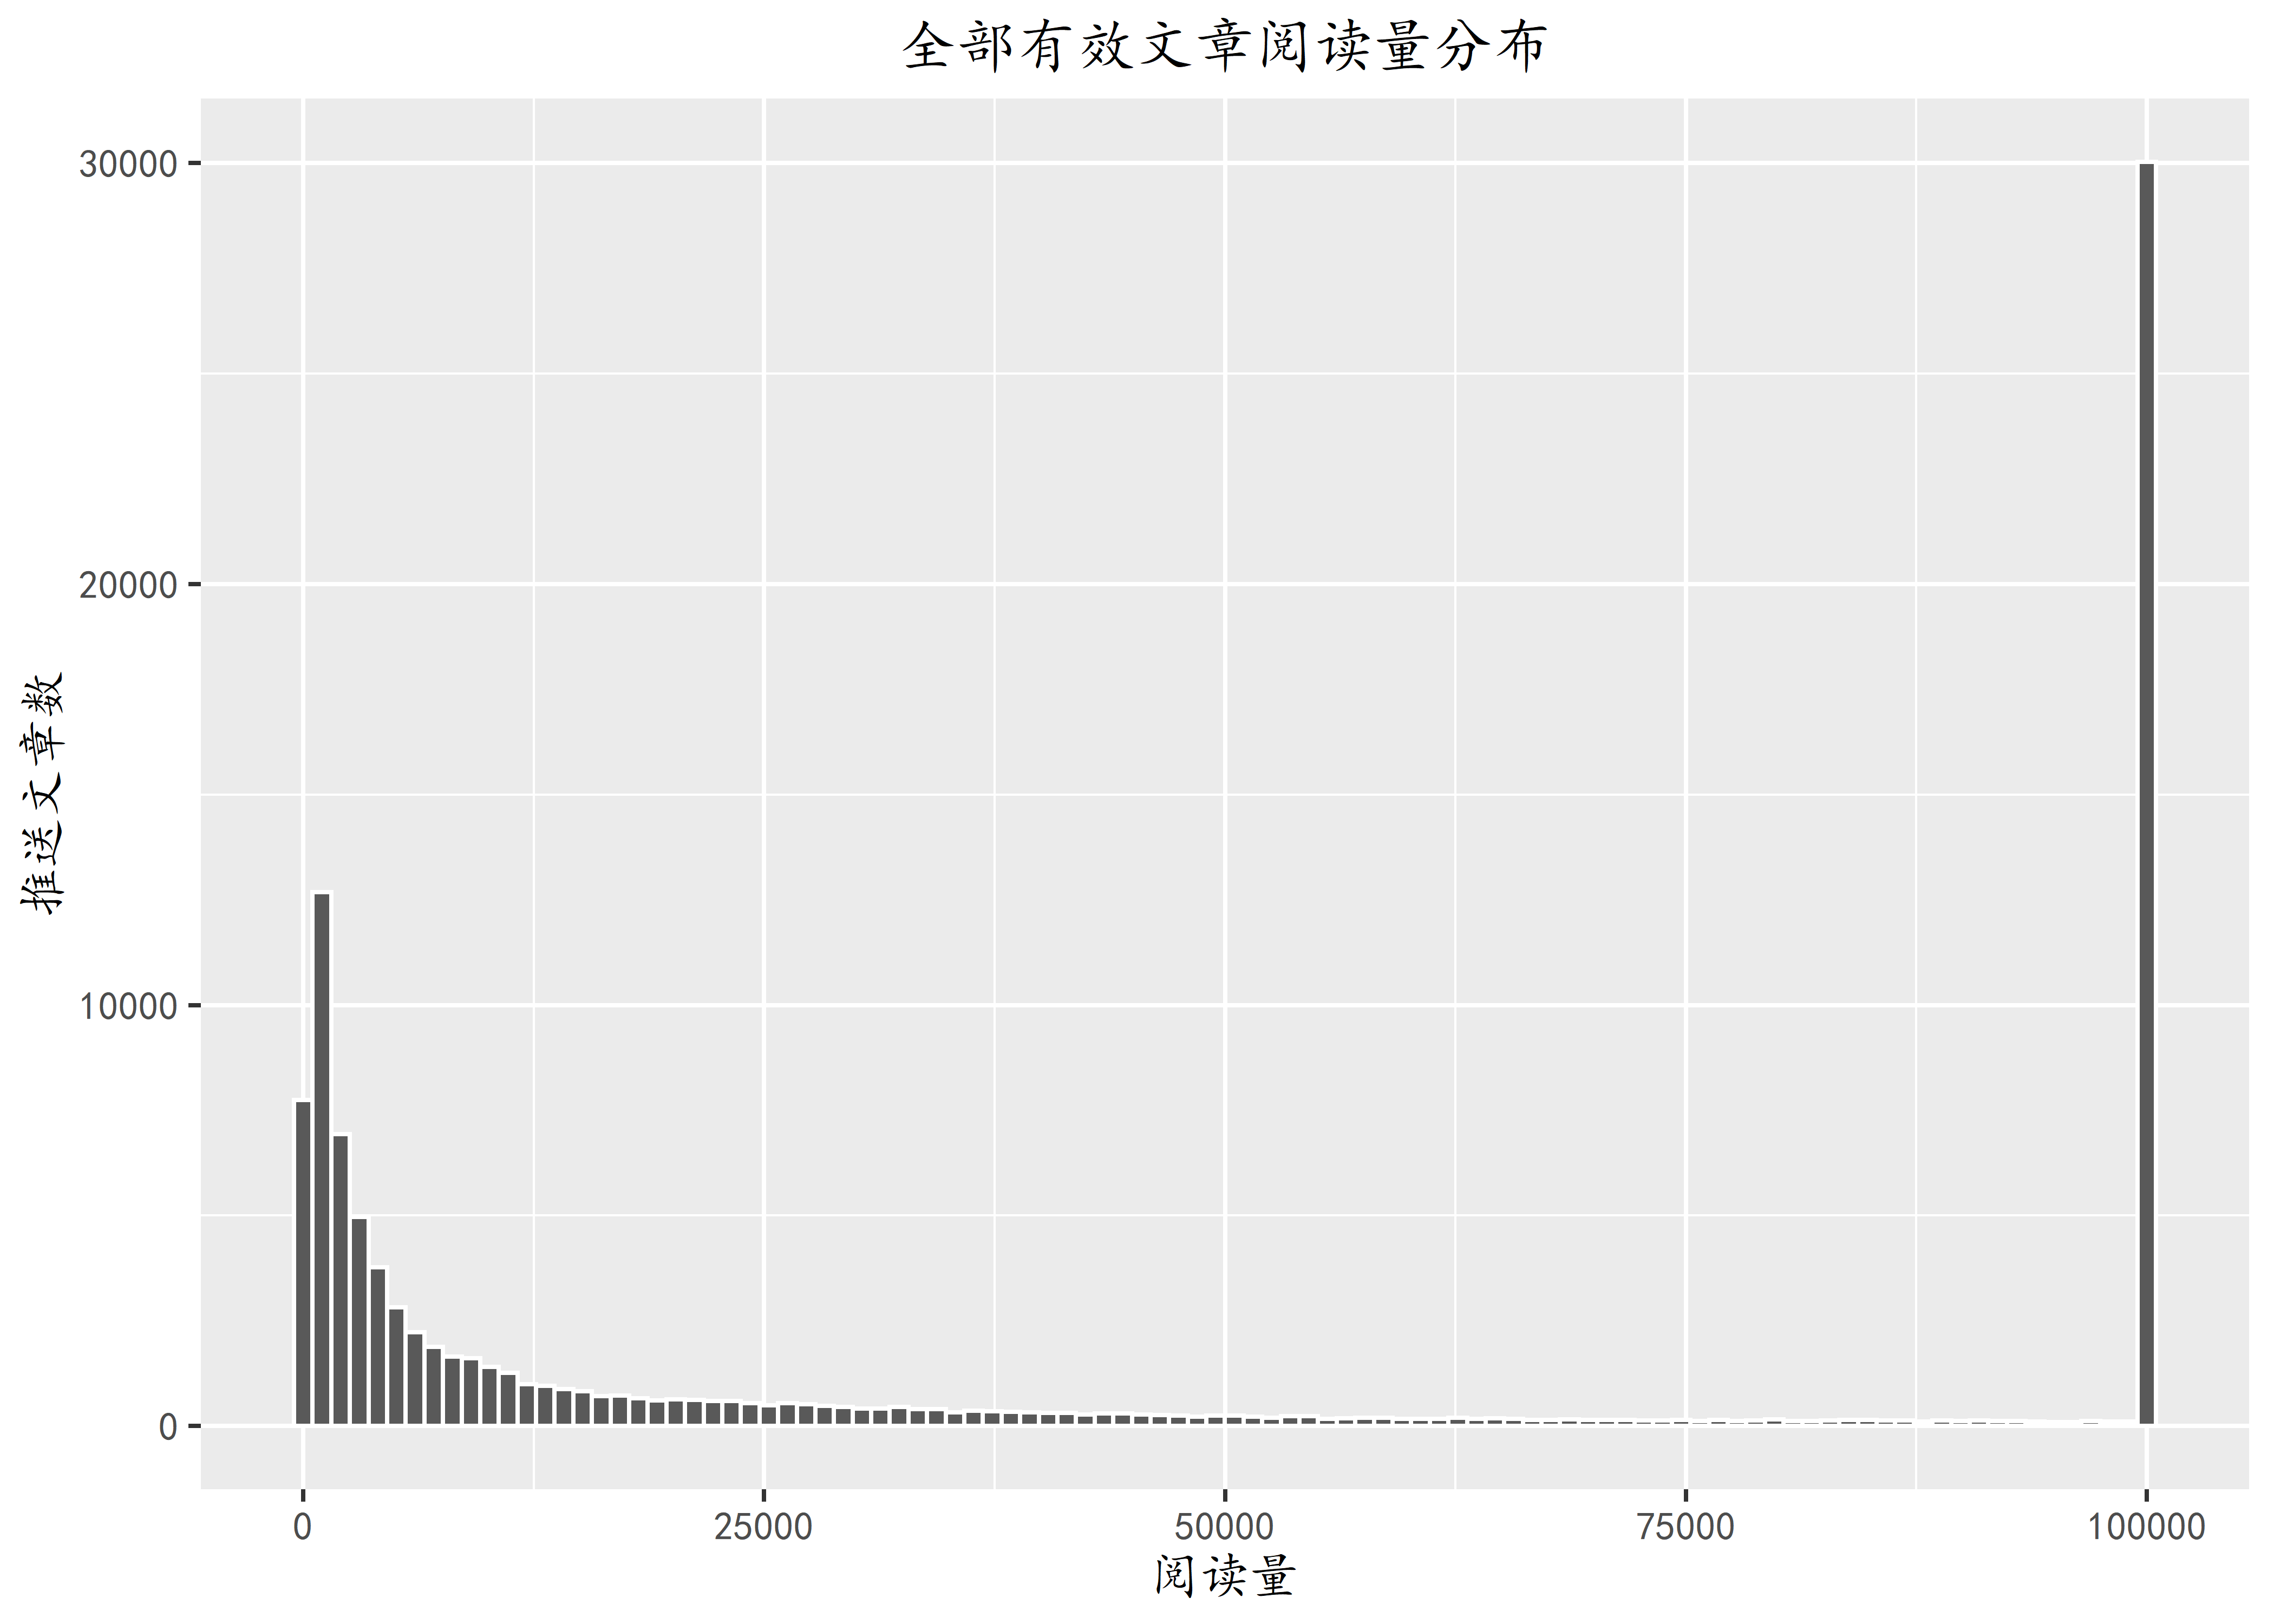
\includegraphics[width=0.9\linewidth]{allR.png}
      \caption{全部推送阅读量分布}
      \label{fig:allR}
    \end{figure}
    \begin{figure}
      \centering
      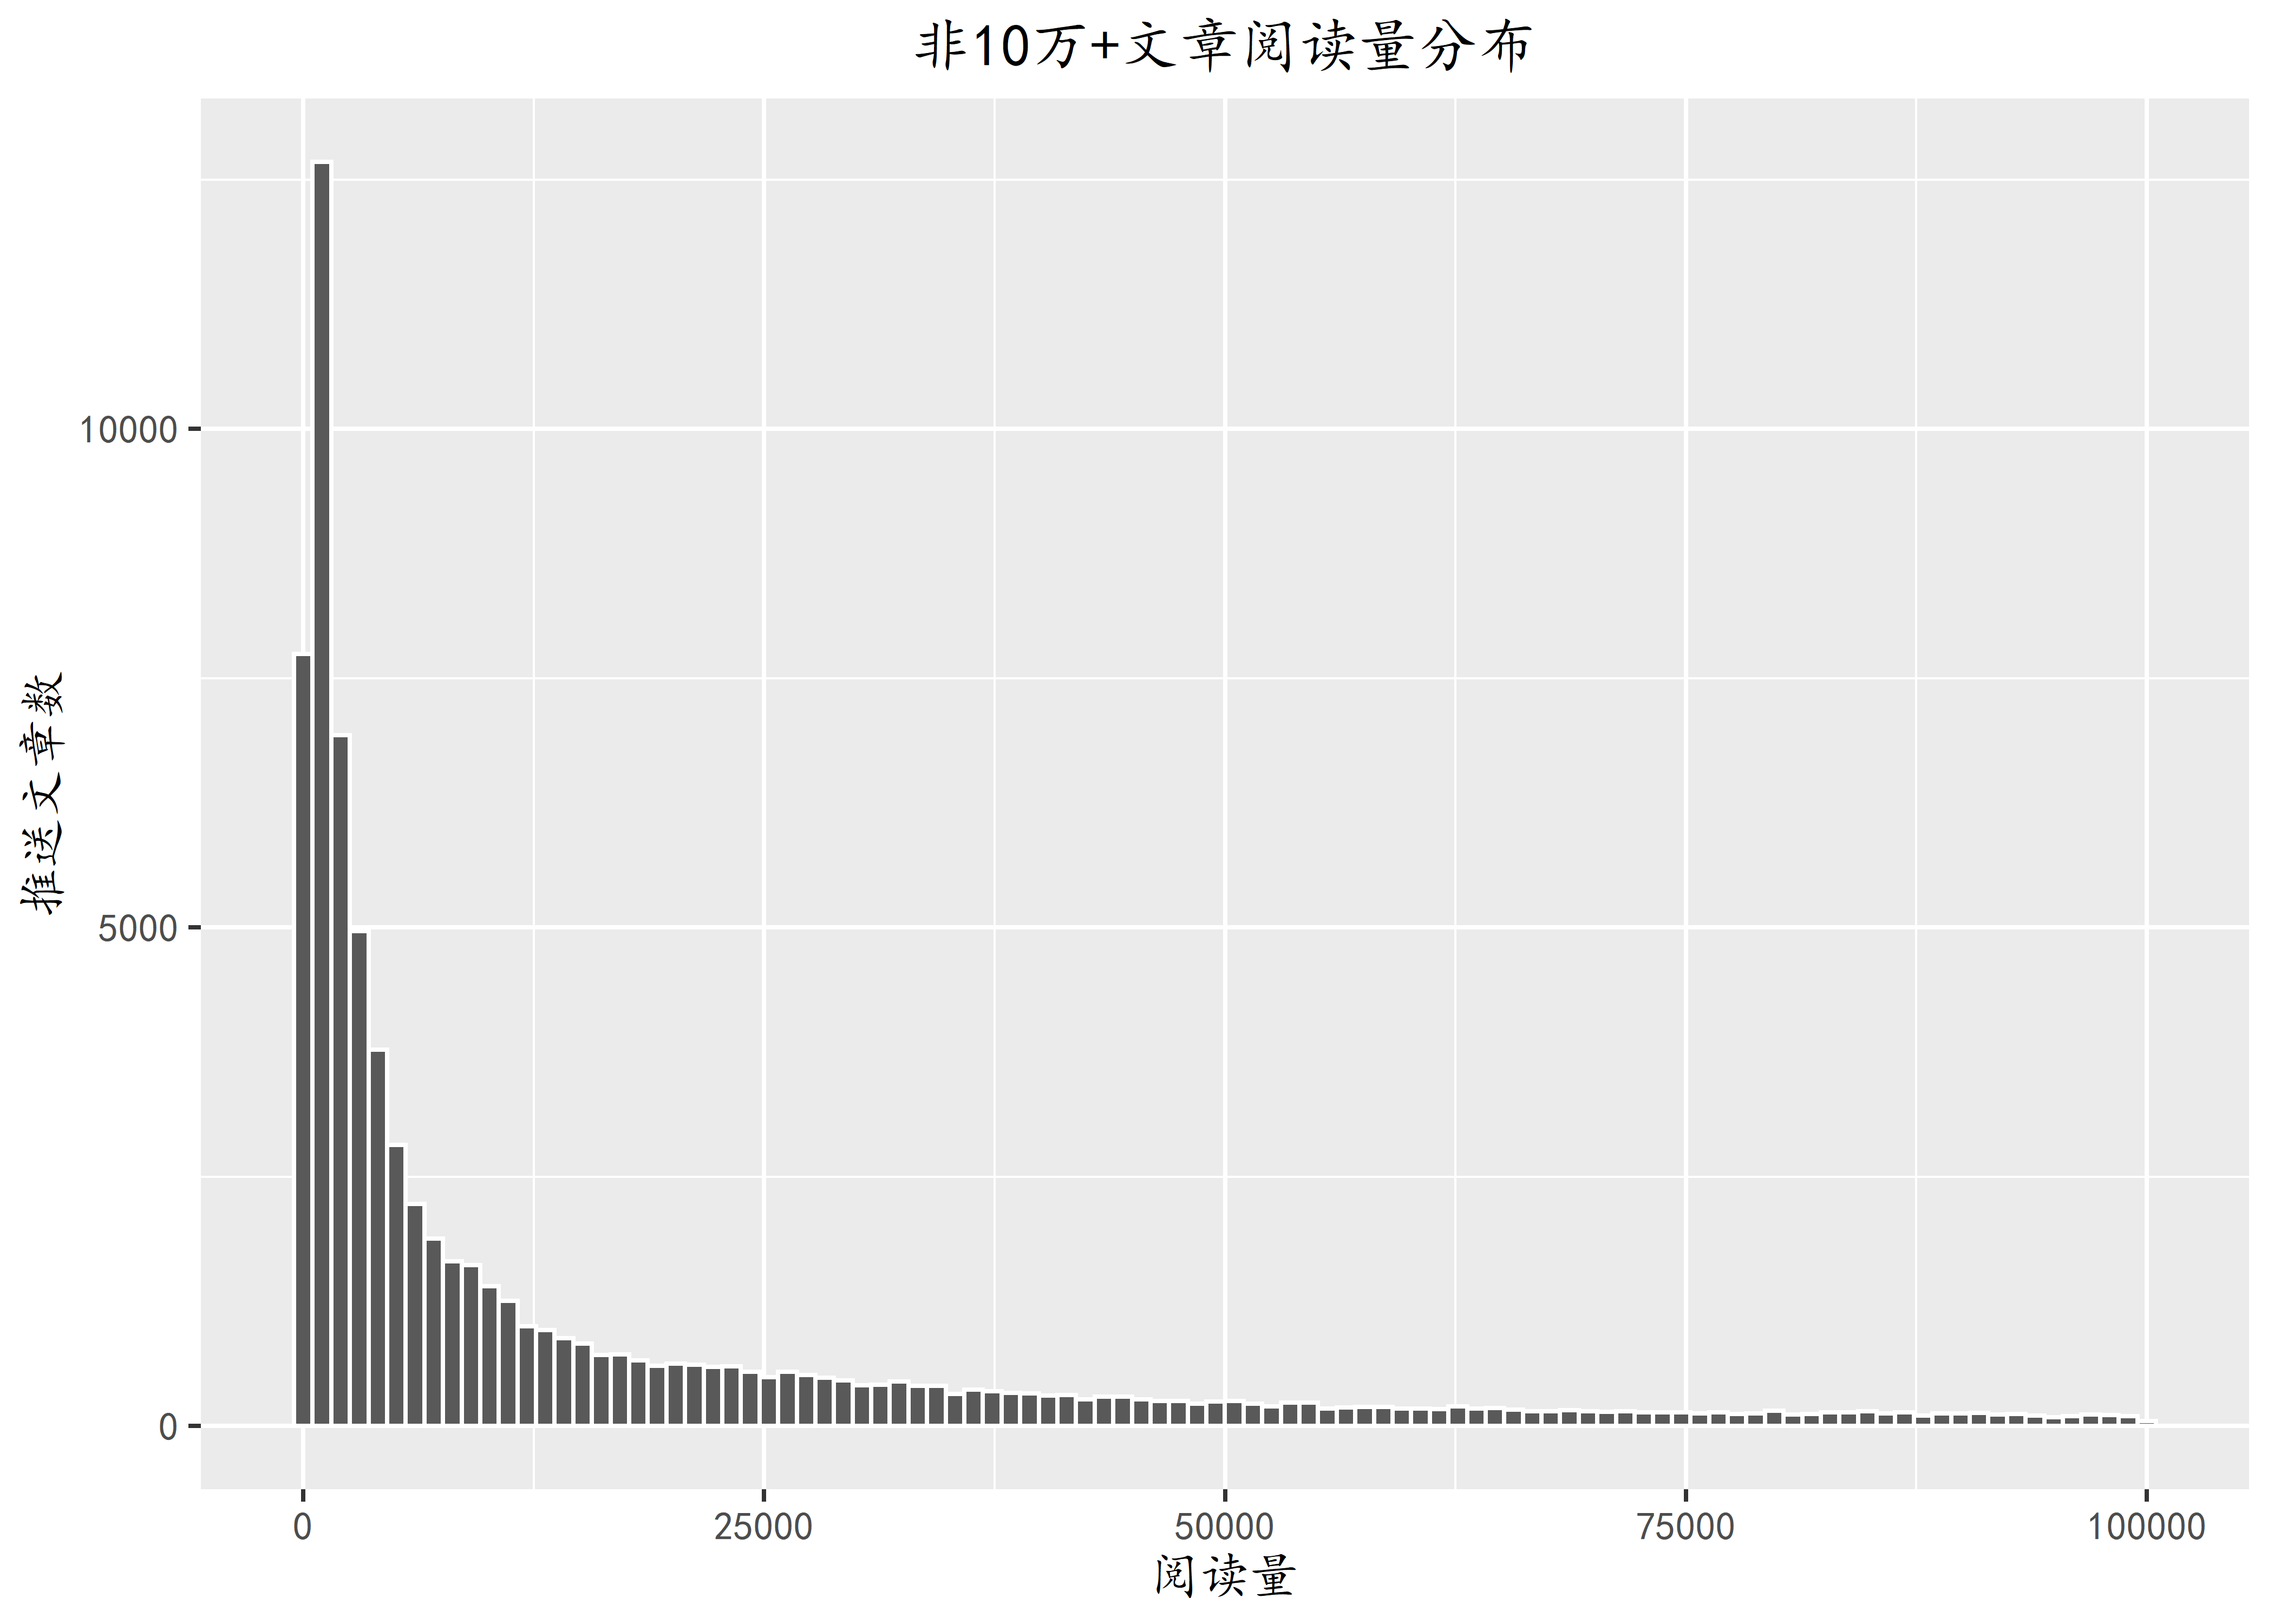
\includegraphics[width=0.9\linewidth]{non10wR.png}
      \caption{非10w+推送阅读量分布}
      \label{fig:nonR}
    \end{figure}

    因此,我们不应以100001估计10w+推送的阅读量,而是应赋予其更大的值。由于泊松尾部的数据方差较大,我们以150000估计其阅读量,以120000估计其在看量。另外,WCI中的平方函数主要是为了调整数据的范围,在我们的研究中并不必要。为了区别这种处理后的系数与WCI的区别,我们记该系数为WPI(Wechat Propagation Index),如\cref{eq:wpi}所示。其中,$R'$为修正后的总阅读数,$Z'$为修正后的总在看数,$R_{max}'$为修正后的最大阅读数,$Z_{max}'$为修正后的最大在看数,$R_t'$为修正后的头条总阅读数,$Z_t'$为修正后的头条总在看数。

    \begin{equation}
      \label{eq:wpi}
      \begin{aligned}
        \text{WPI} &= 0.3\left[0.85 \ln (\frac{R'}{d} + 1)+ 0.15 \ln (\frac{10Z'}{d} + 1)\right] \\
                   &+ 0.3\left[0.85 \ln (\frac{R'}{n} + 1)+ 0.15 \ln (\frac{10Z'}{n} + 1)\right] \\
                   &+ 0.1\left[0.85 \ln (R_{max}' + 1)+ 0.15 \ln (10Z_{max}' + 1)\right] \\
                   &+ 0.3\left[0.85 \ln (\frac{R_t'}{d} + 1)+ 0.15 \ln (\frac{10Z_t'}{d} + 1)\right] \\
      \end{aligned}
    \end{equation}
    另记单片推送系数为PPI(Post Propagation Index),计算方式如\cref{eq:ppi}所示。其中,$R$为该推送阅读量,$Z$为该推送在看量。
    \begin{equation}
      \label{eq:ppi}
      \text{PPI} = 0.85 \ln (\frac{R}{d} + 1)+ 0.15 \ln (\frac{10Z}{d} + 1)
    \end{equation}
    \section{研究发现及结果解释}
    \subsection{公众号主题效力分析}
    这部分我们聚焦各政府发布公众号。首先应对各公众号进行主题分解,分解结果部署在网络上,可以通过访问\url{https://nogeek-static.netlify.com/gov/公众号名称/#lambda=0.2}查看,该网页的生成采用了LDAvis包\cite{sievert2014ldavis}。例如,访问\url{https://nogeek-static.netlify.com/gov/上海发布/#lambda=0.2},可见如\cref{fig:shanghai-vis}所示界面。图中,左侧的圆圈代表了10个主题在两个主成分下的分布情况,圆圈距离越近代表主题越接近。点击各个圆圈,可以查看该主题下的成分词。每个主题均由若干主题成分词描述,其排序综合考虑了该主题词在当前主题下的频率绝对值及相对全部文档中的频率的相对值,选择系数$\lambda=0.2$代表更多地考虑主题词的相对值,即该主题的特色词。例如,\cref{fig:shanghai-vis}中的主题1包括以下词组:发展,创新,李强,推动,产业,习近平,全球……。可见,该主题主要是政治政策。
  
    \begin{figure}
      \centering
      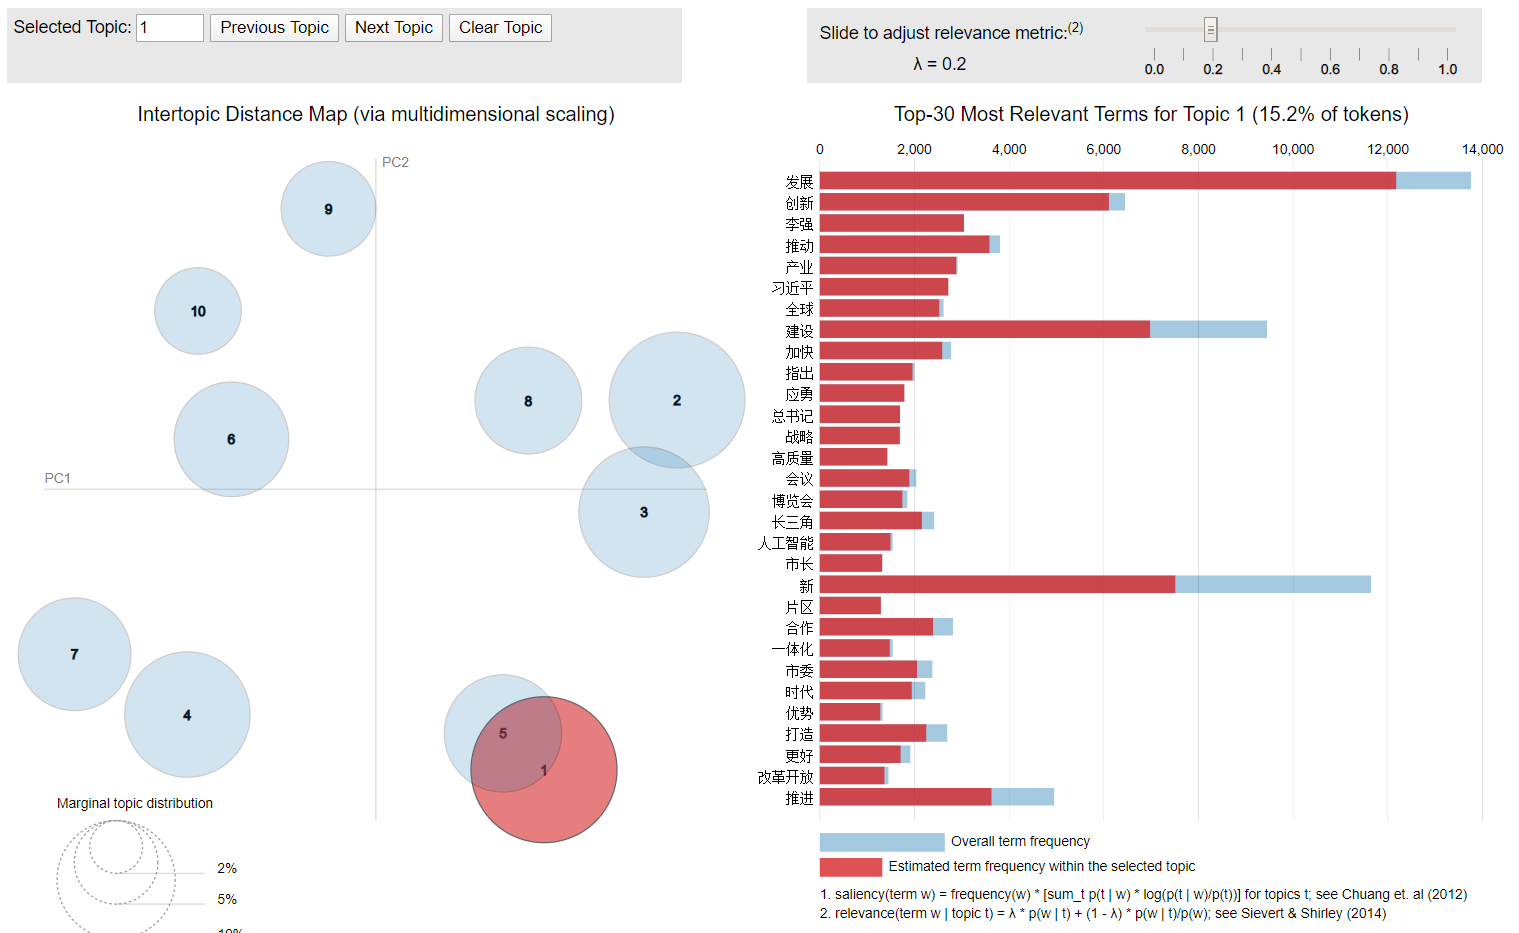
\includegraphics[width=0.9\linewidth]{shanghai-vis.png}
      \caption{“上海发布”公众号主题分解可视化}
      \label{fig:shanghai-vis}
    \end{figure}

    主题分解后,可以得到该公众号下每篇推送关于每个主题$i$的权重$T_i$,该权重有约束$$\sum_{i=1}^{10}T_i=1$$,权重$T_i$表示了该篇推送和主题$i$的相关程度。

    \cref{fig:长沙发布-box}到\cref{fig:深圳发布-box}展示了政府发布公众号的折算传播力度在各主题下的分布情况,用箱图表示。对于一篇推送$p$,折算结果$R_i(p)$计算如\cref{eq:zhesuan}所示。
    \begin{equation}
      \label{eq:zhesuan}
      R_i(p) = T_i\text{PPI}(p)
    \end{equation}
    $R_i(p)$越大,代表该主题的折算推送传播效力越高,即该主题下的推送更容易被传播。
    
    由于绘图的限制,此处每个主题均以排序第一的代表词表示,具体主题词组则需查询\url{https://nogeek-static.netlify.com/gov/公众号名称/#lambda=0.2}。对\cref{fig:上海发布-box}来说,“报名”代表的主题(报名,考生,招生,考试,招聘,岗位,报考,面试,录取,资格,专业)传播力显然最低,而“号线”代表的主题(号线,地铁,景区,免费,虹桥,票价,客流,铁路,门票,列车,高速)、“垃圾”代表的主题(垃圾,分类,部门,监管,住房,审批,保障,服务,规范,整治,处置,养老)传播力则显然更高。这也意味着,在“上海发布”公众号,交通话题和民生话题更受受众关注,而公众或许不太会在这个公众号上关注招考相关的信息。

    % 
\begin{figure}
  \centering
  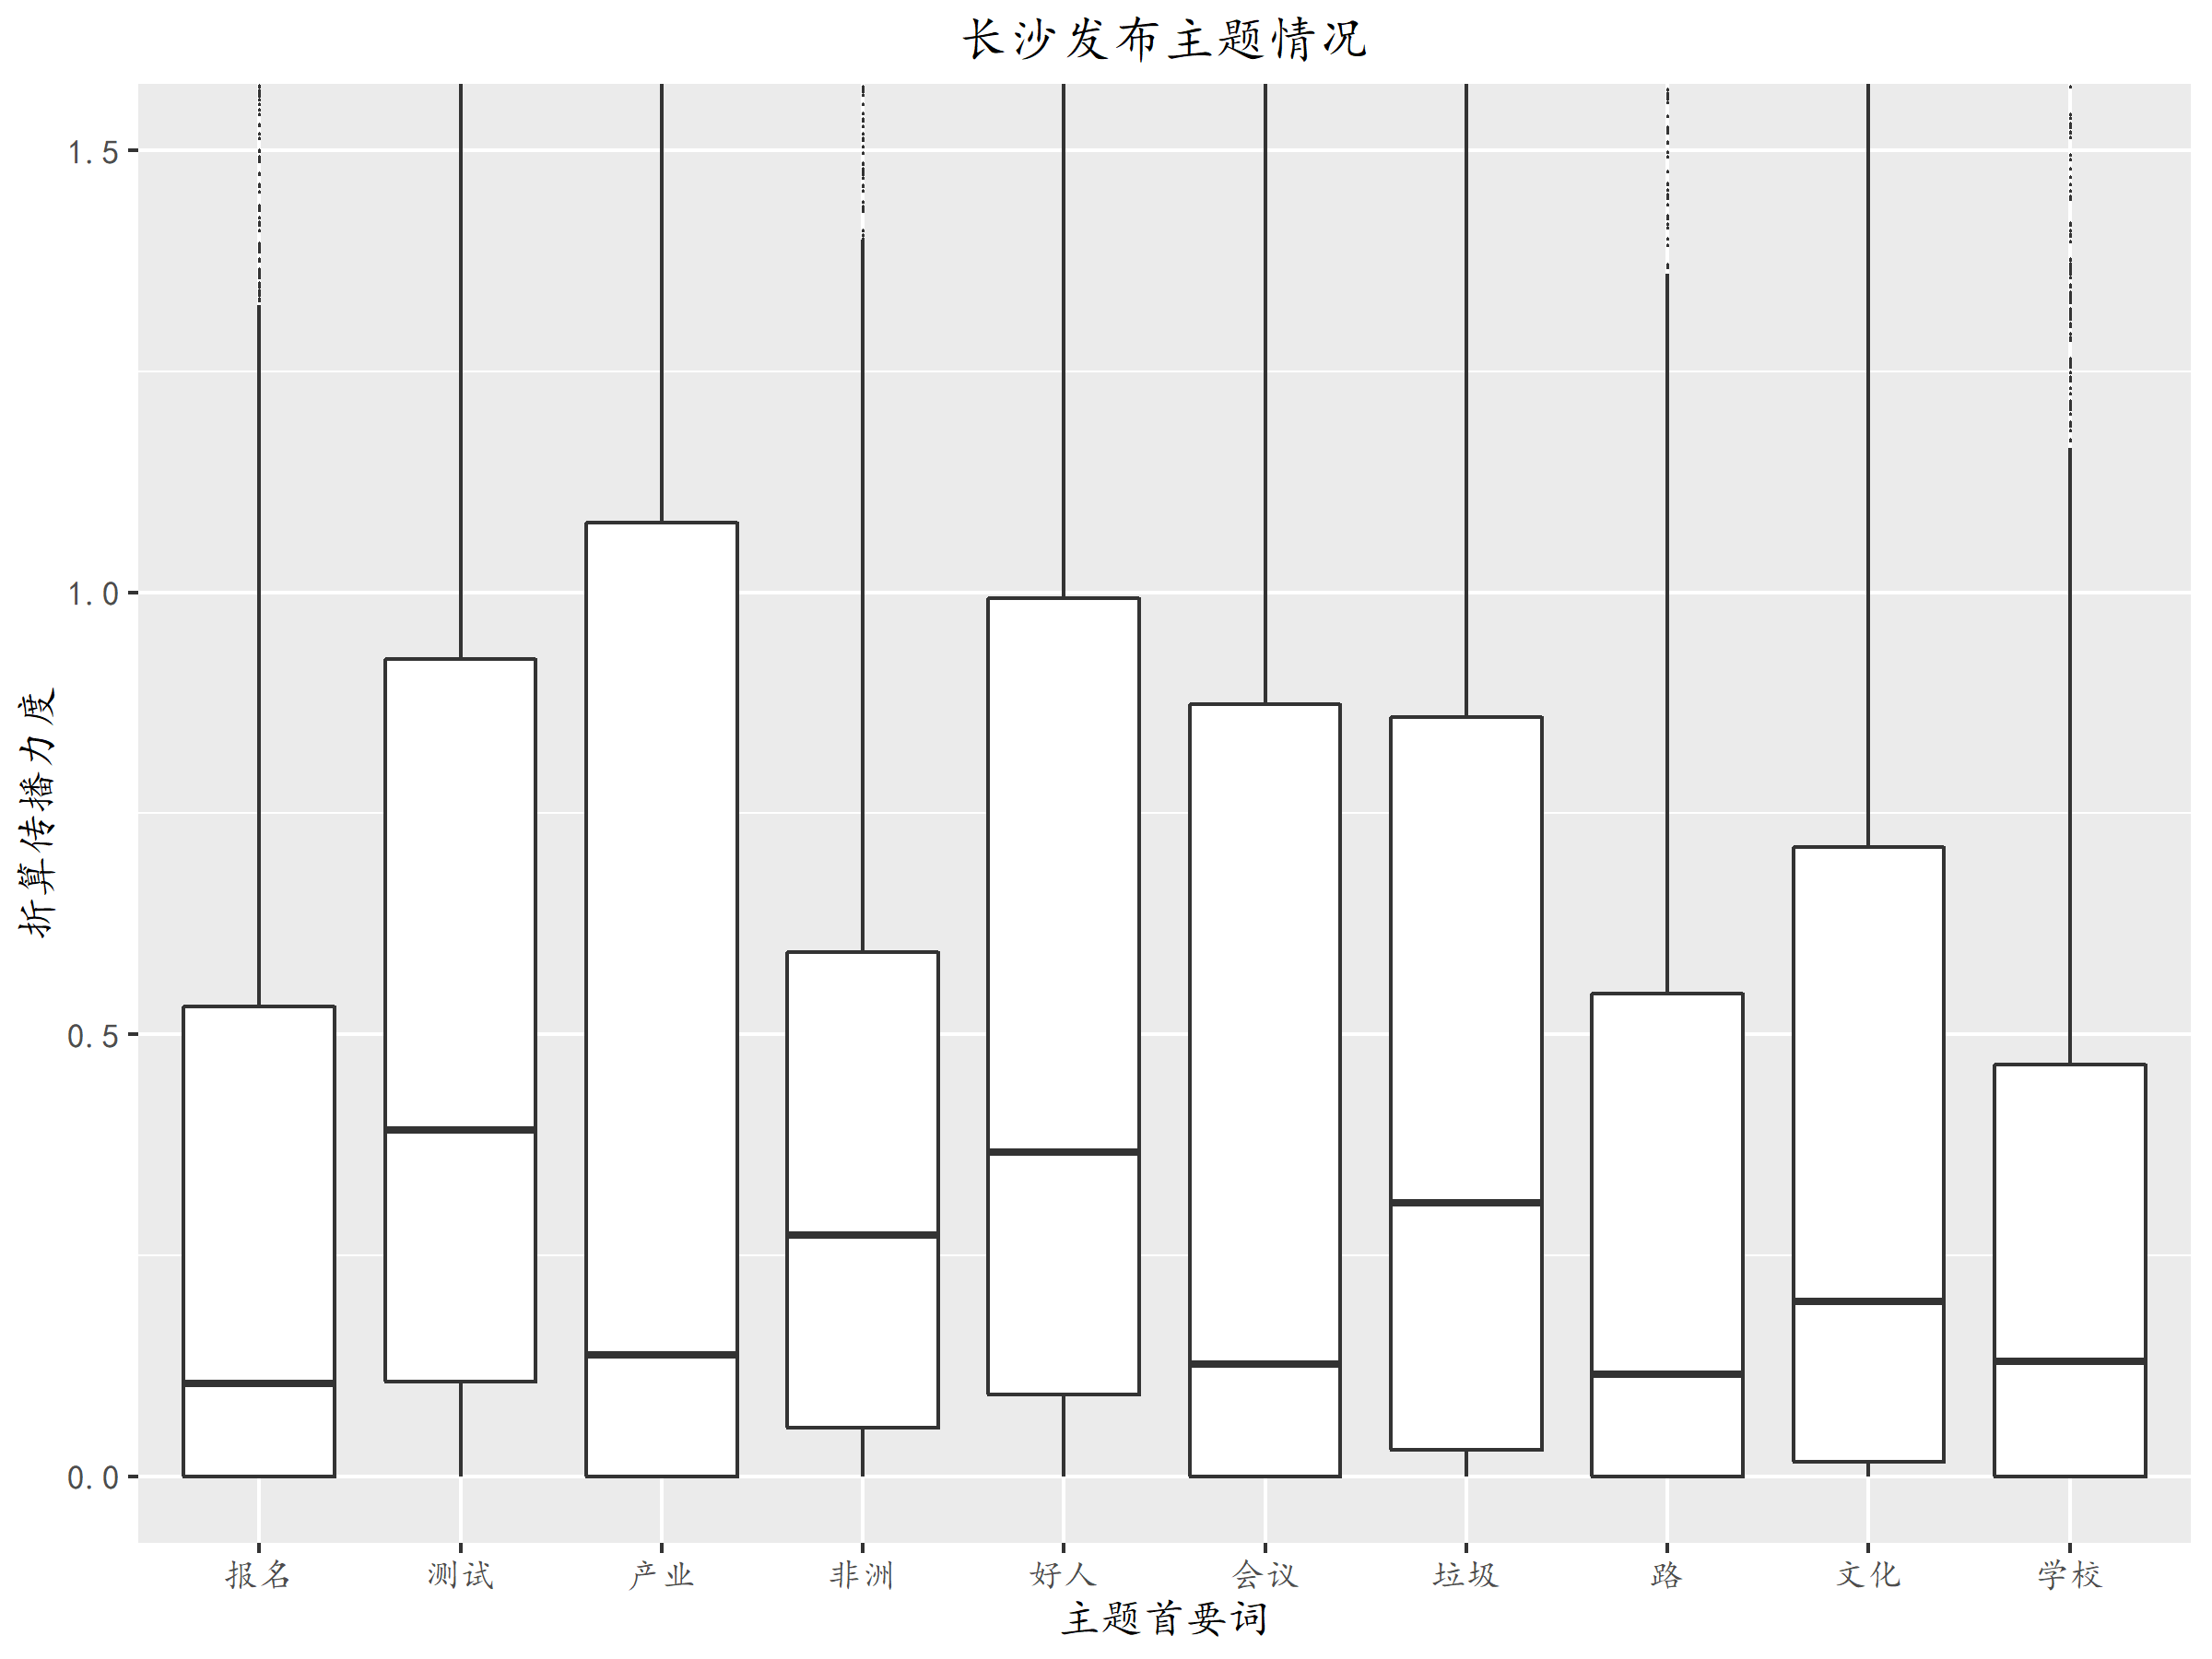
\includegraphics[width=0.9\linewidth]{长沙发布.png}
  \caption{"长沙发布"公众号各主题下推送传播效力分布}
  \label{fig:长沙发布-box}
\end{figure}

\begin{figure}
  \centering
  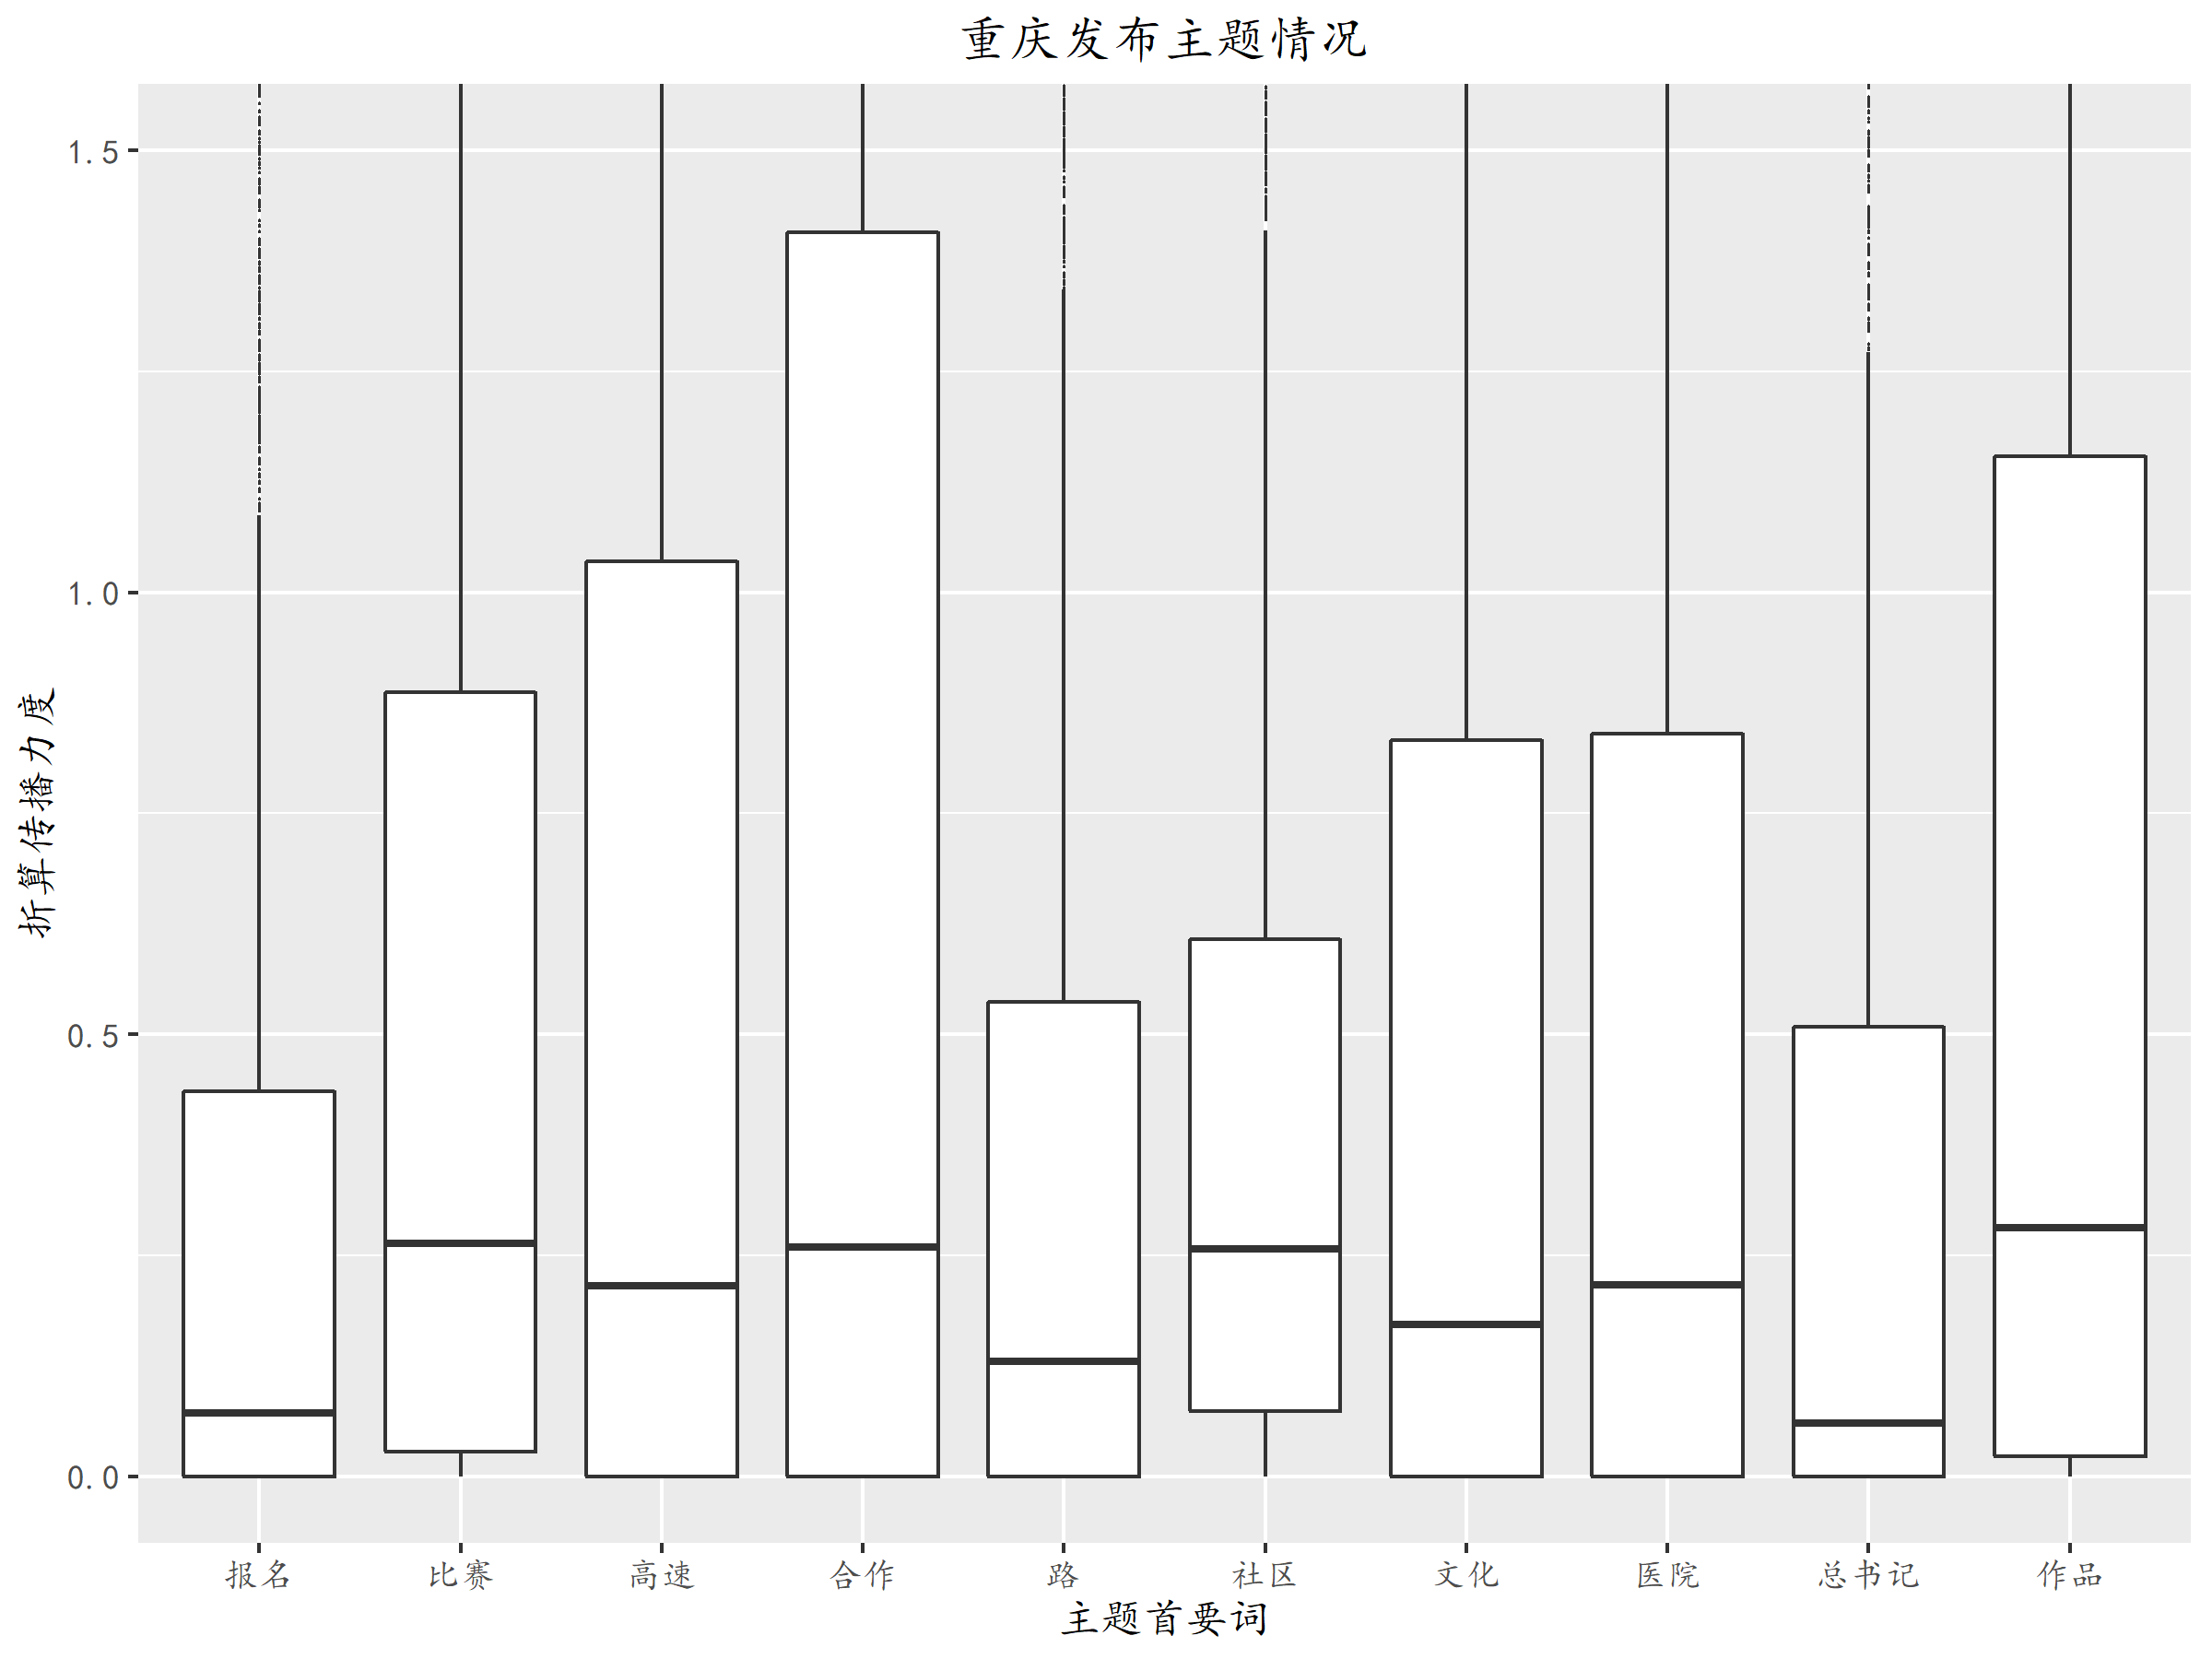
\includegraphics[width=0.9\linewidth]{重庆发布.png}
  \caption{"重庆发布"公众号各主题下推送传播效力分布}
  \label{fig:重庆发布-box}
\end{figure}

\begin{figure}
  \centering
  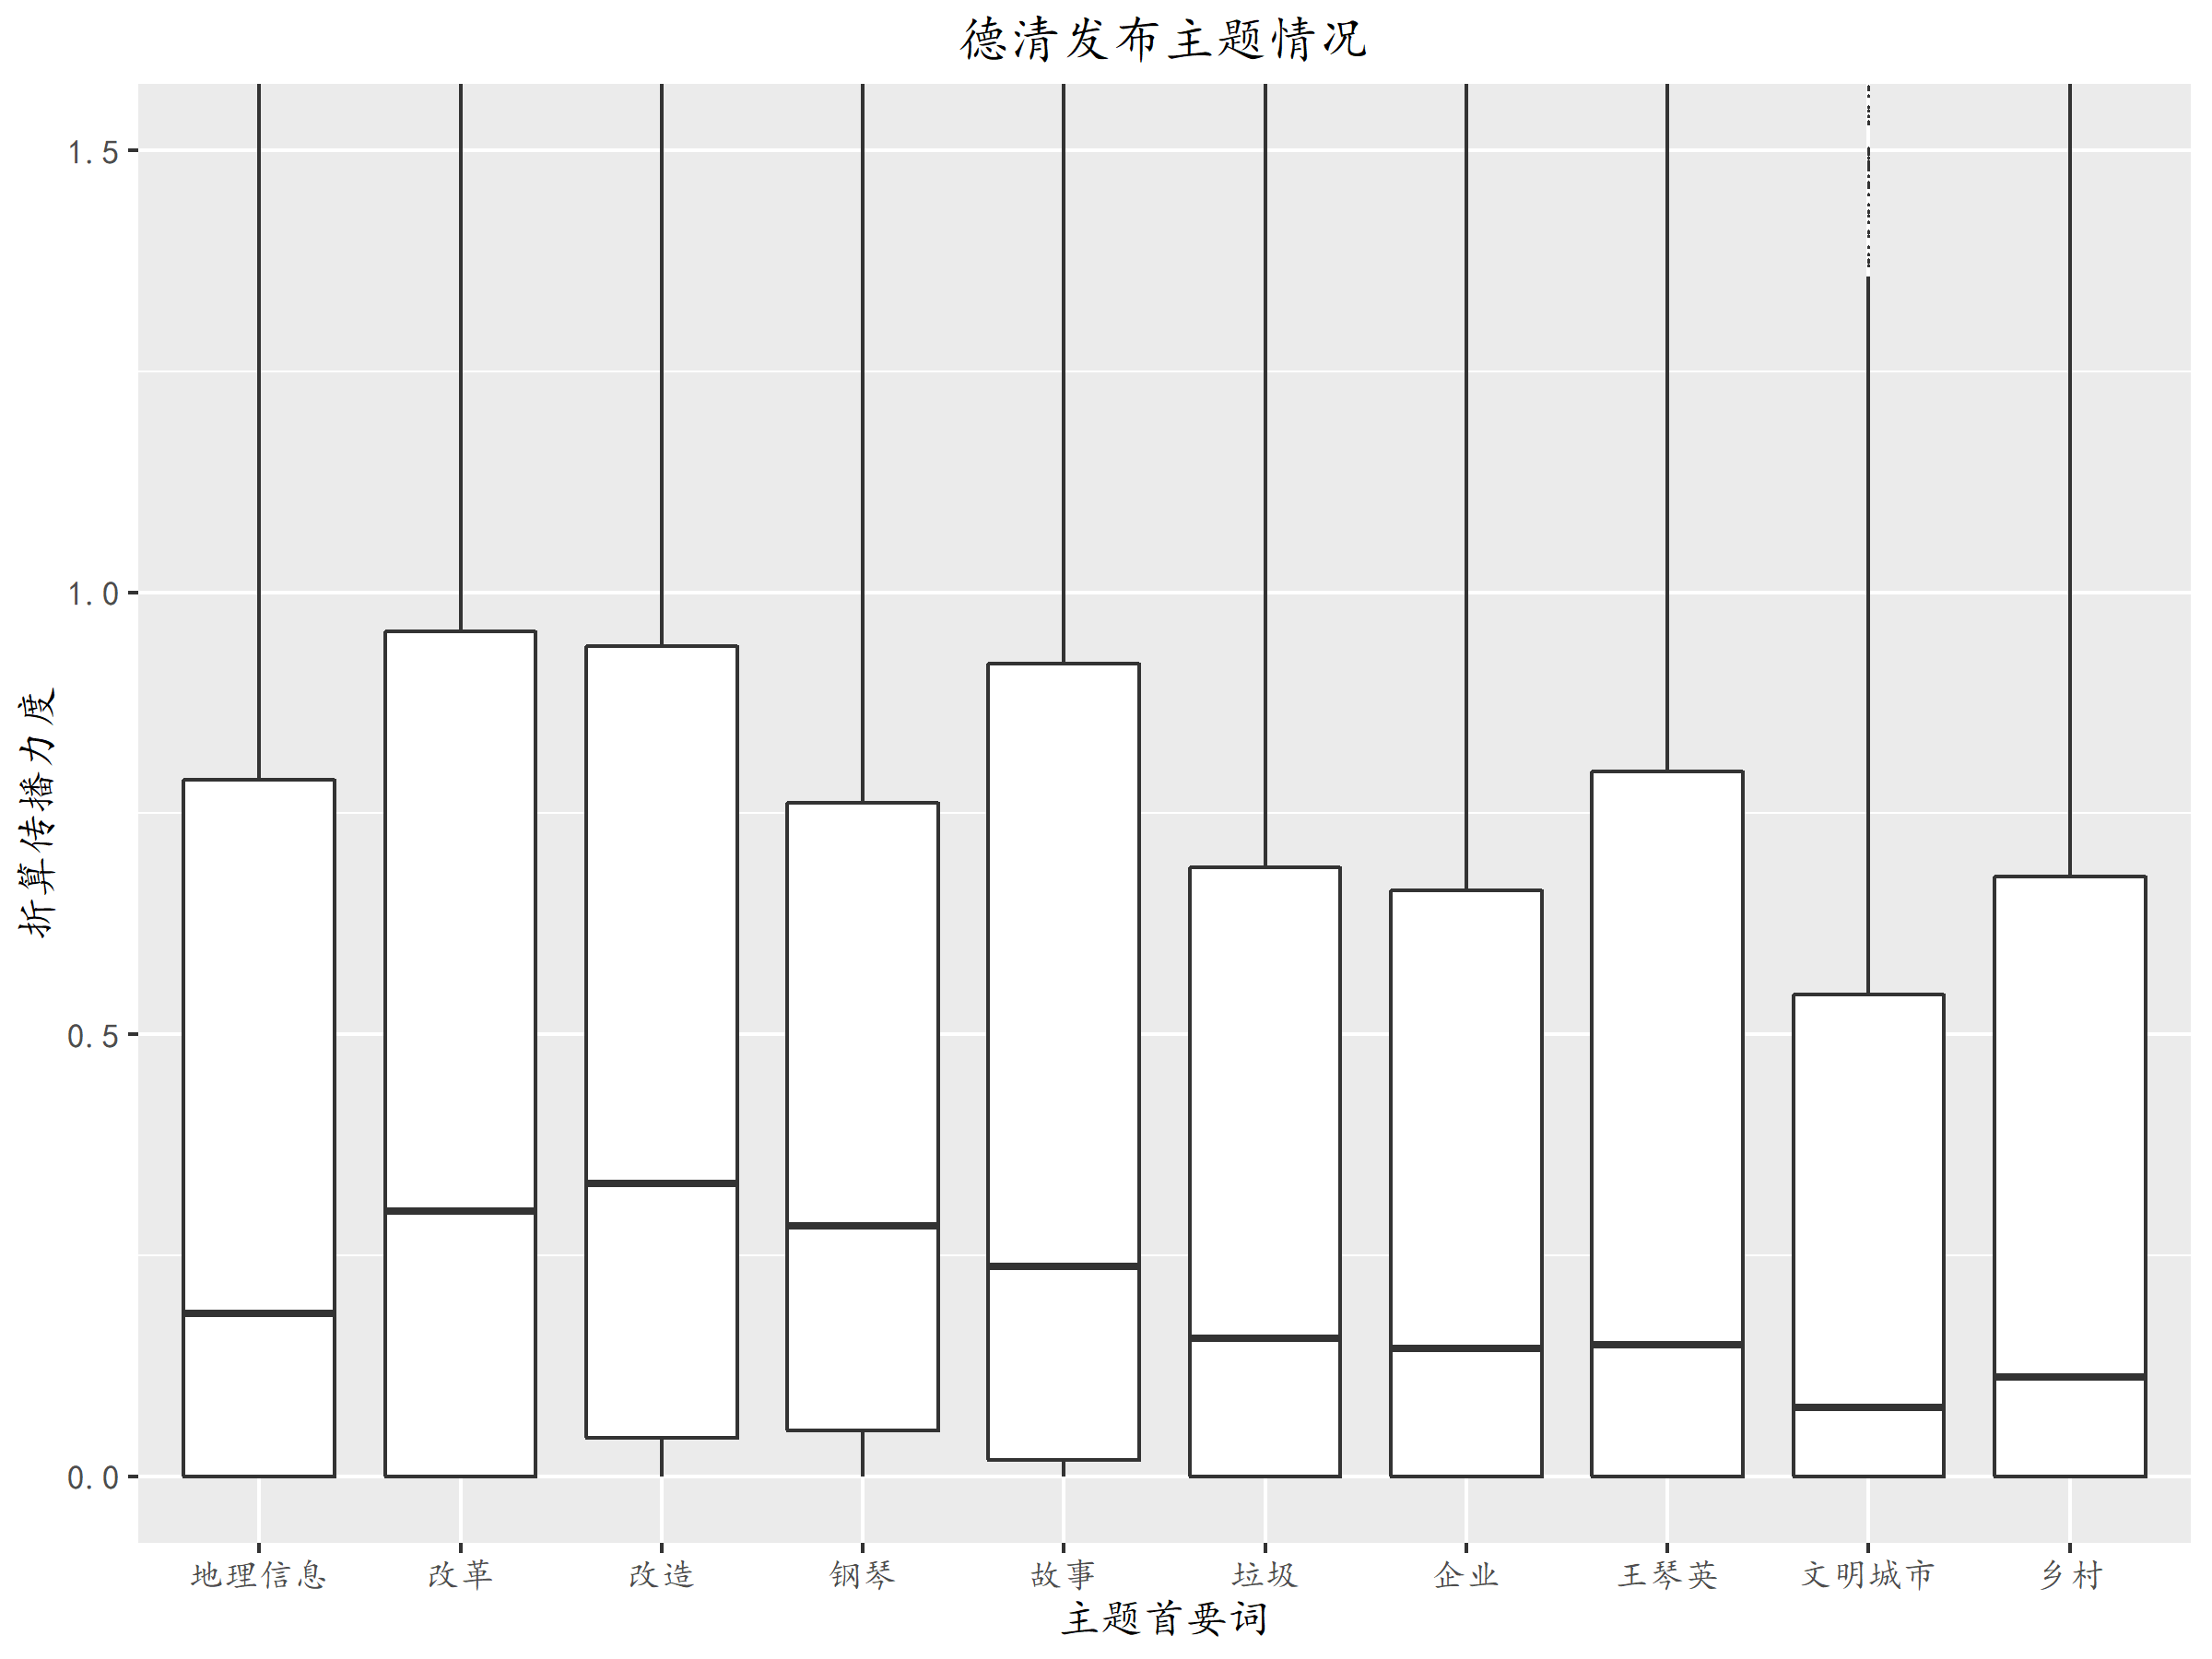
\includegraphics[width=0.9\linewidth]{德清发布.png}
  \caption{"德清发布"公众号各主题下推送传播效力分布}
  \label{fig:德清发布-box}
\end{figure}

\begin{figure}
  \centering
  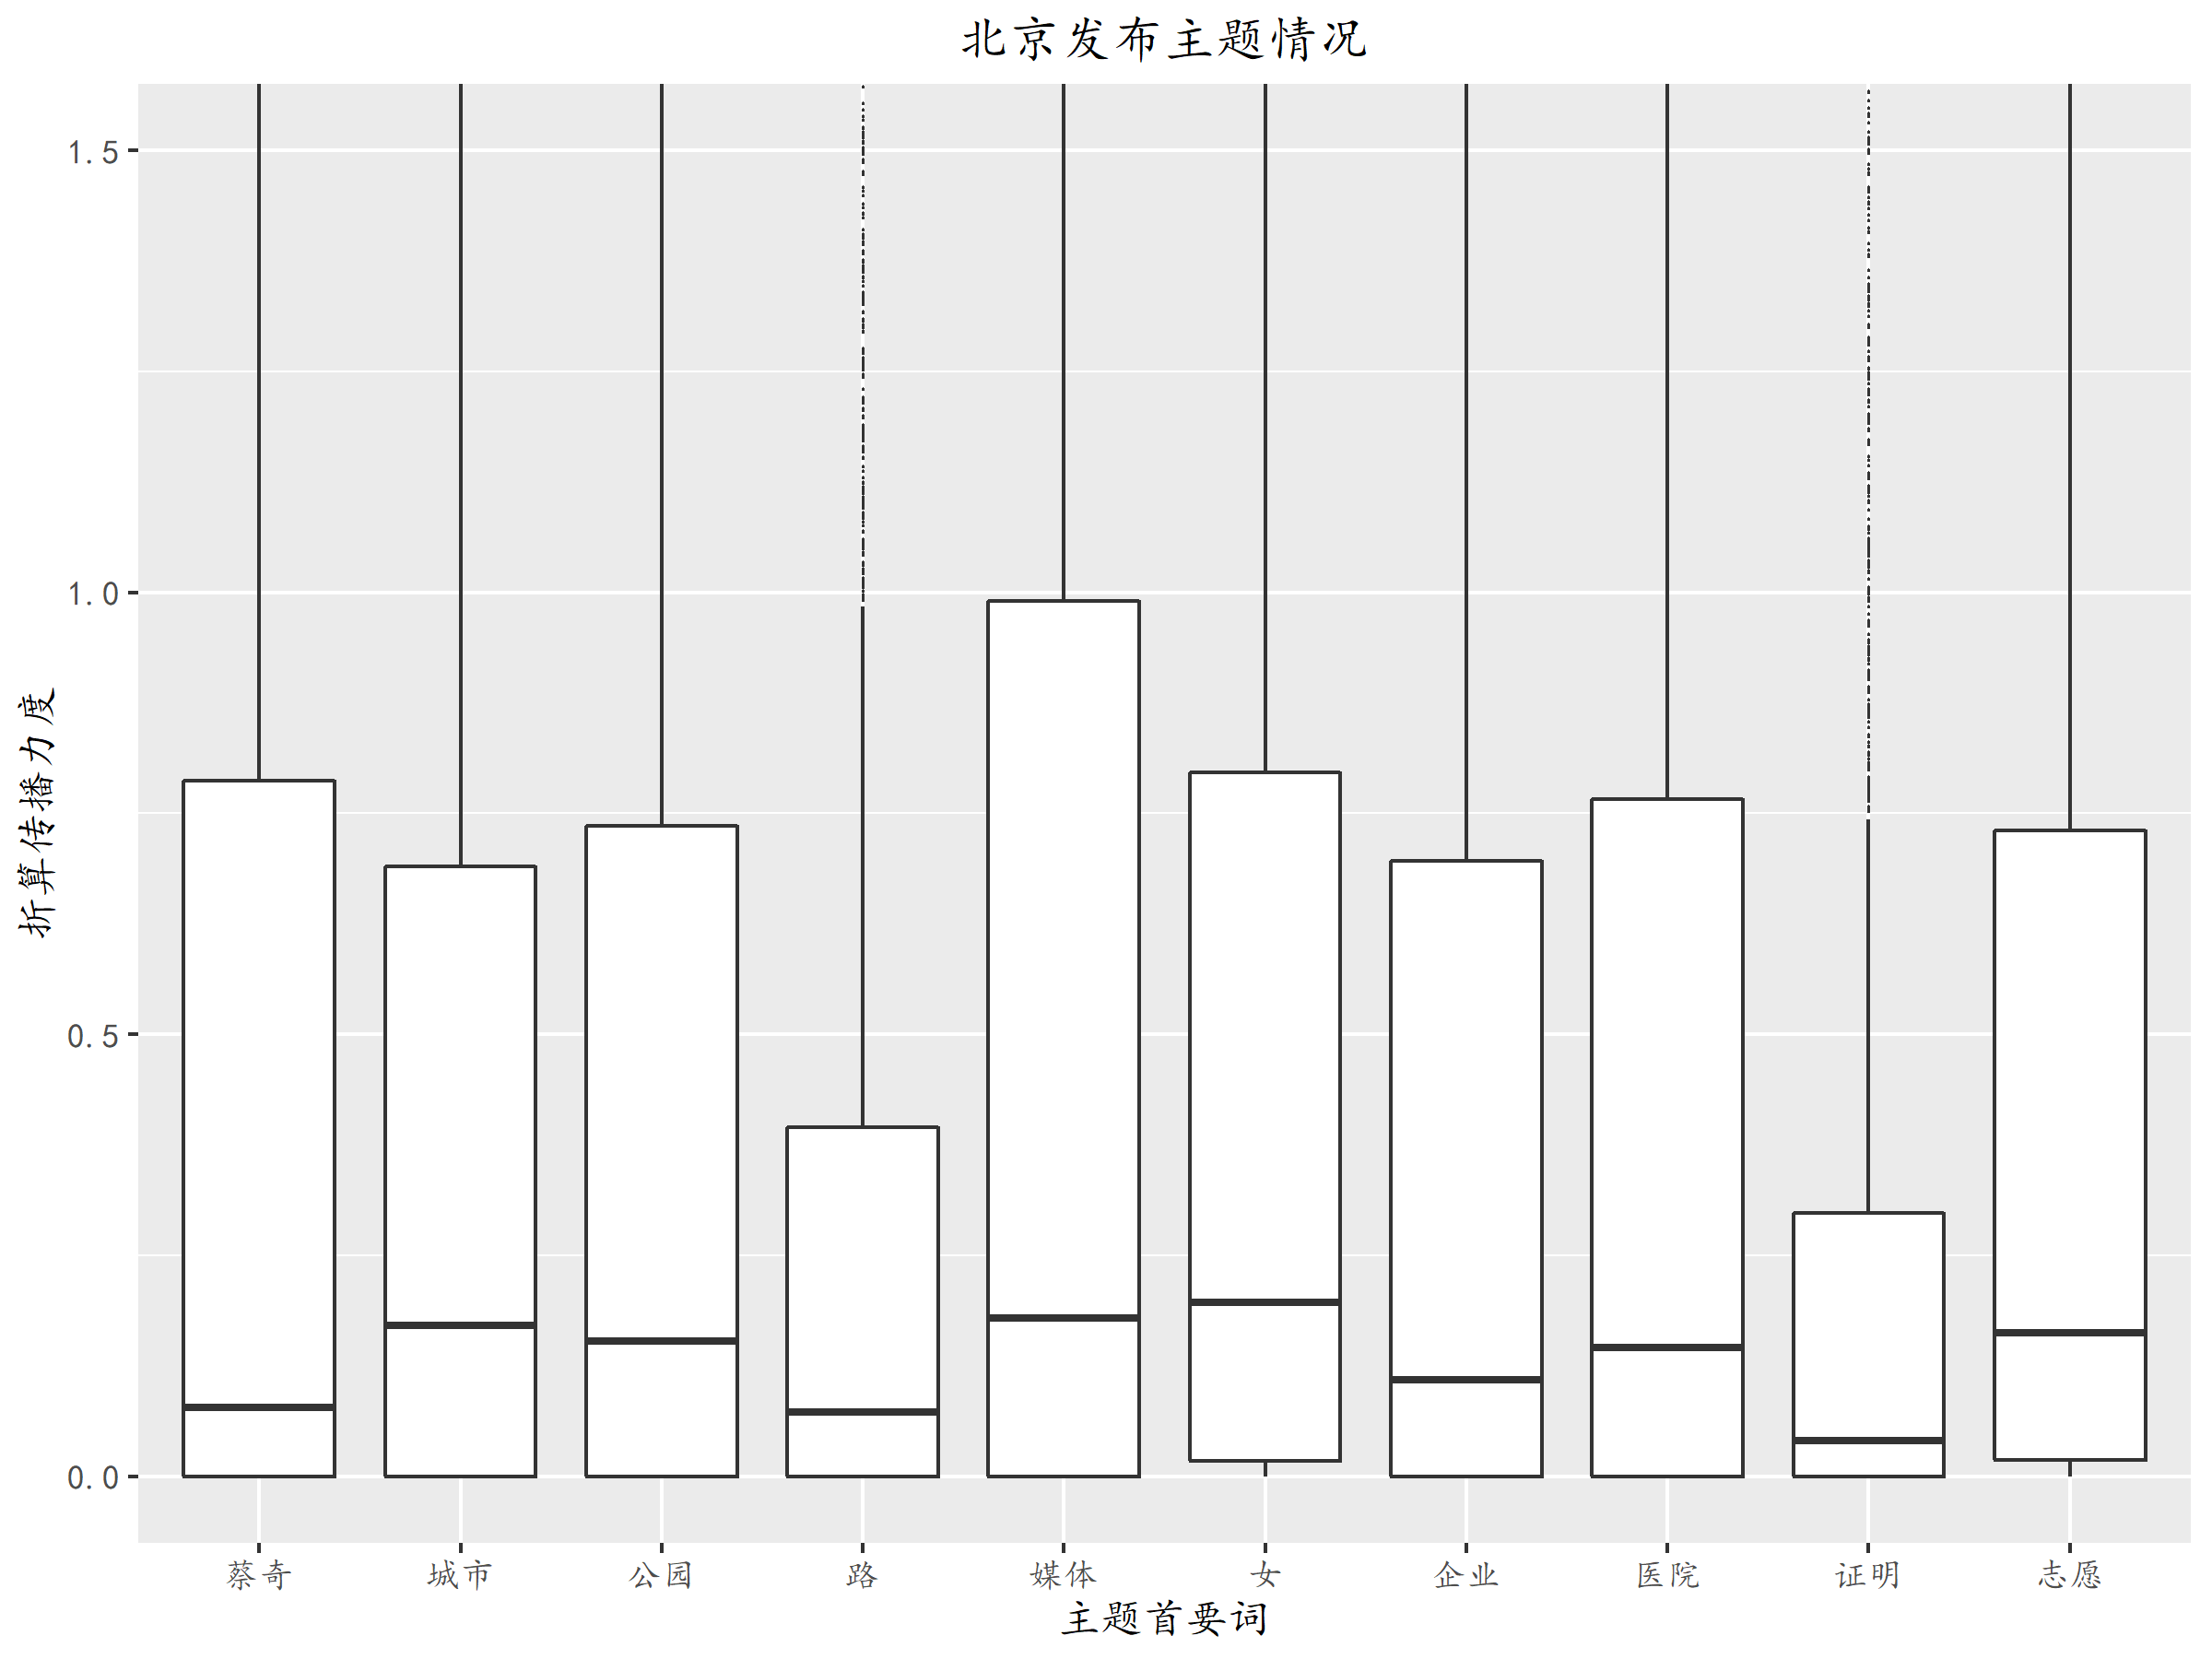
\includegraphics[width=0.9\linewidth]{北京发布.png}
  \caption{"北京发布"公众号各主题下推送传播效力分布}
  \label{fig:北京发布-box}
\end{figure}

\begin{figure}
  \centering
  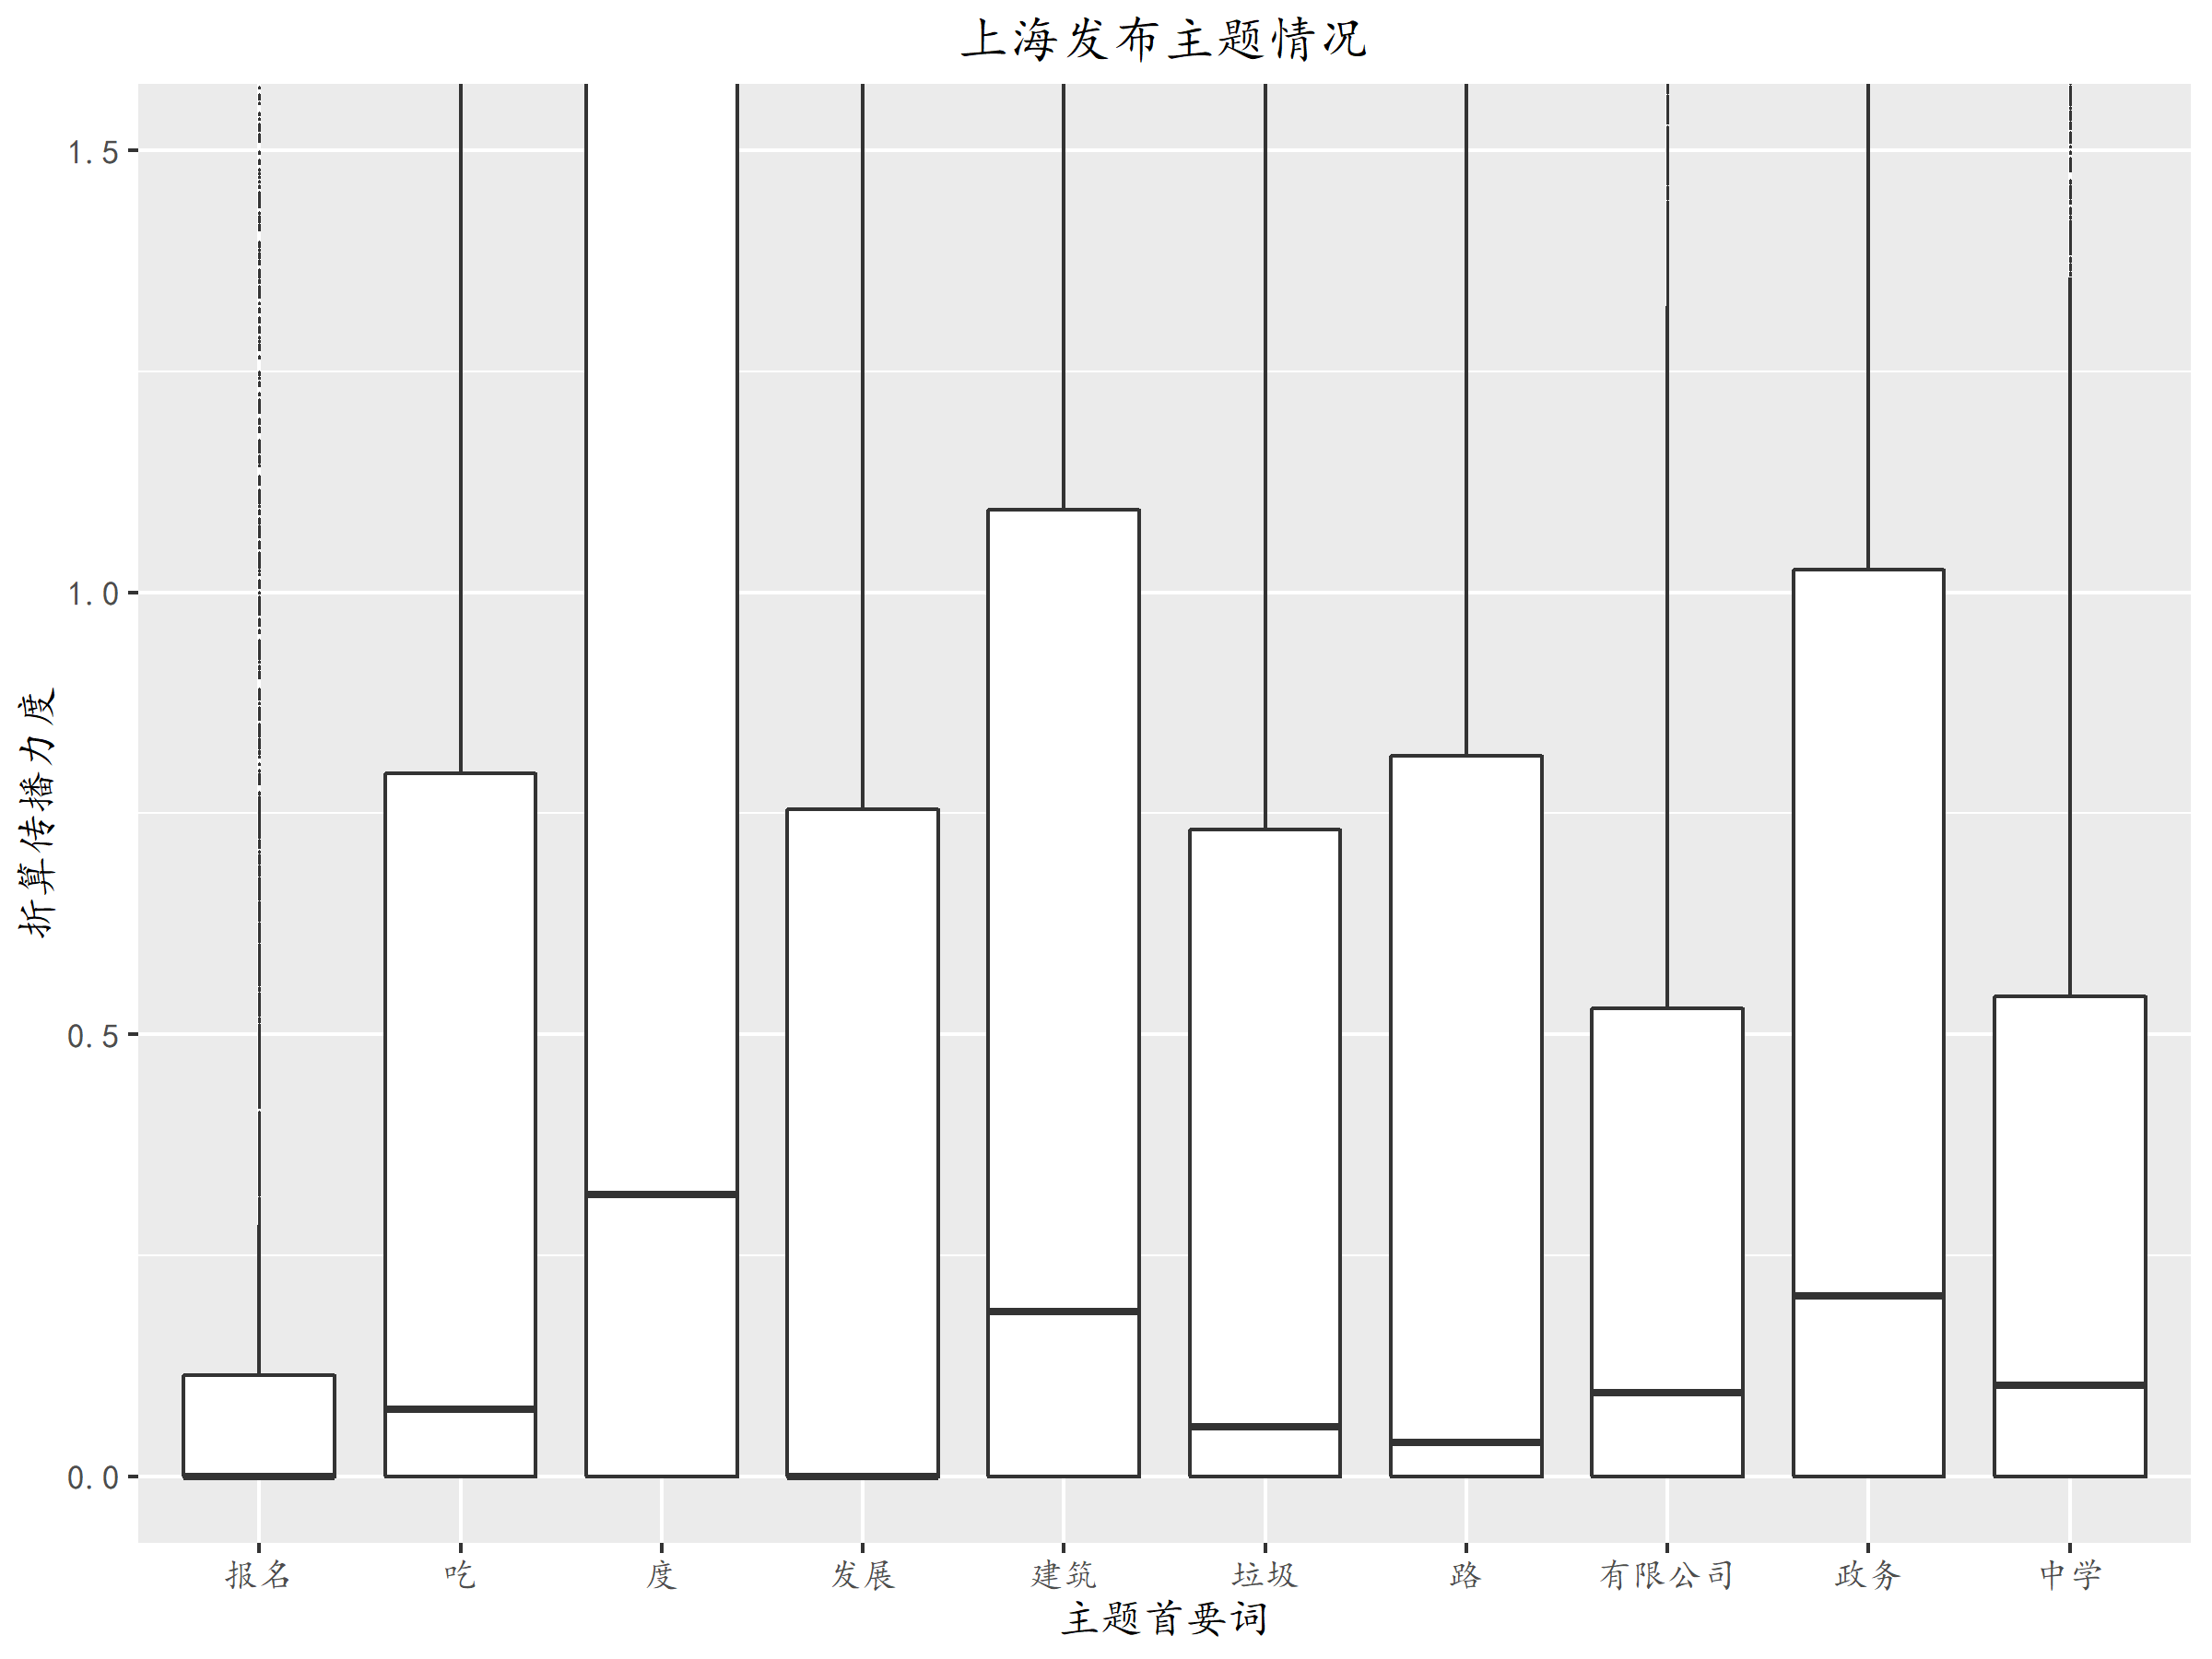
\includegraphics[width=0.9\linewidth]{上海发布.png}
  \caption{"上海发布"公众号各主题下推送传播效力分布}
  \label{fig:上海发布-box}
\end{figure}

\begin{figure}
  \centering
  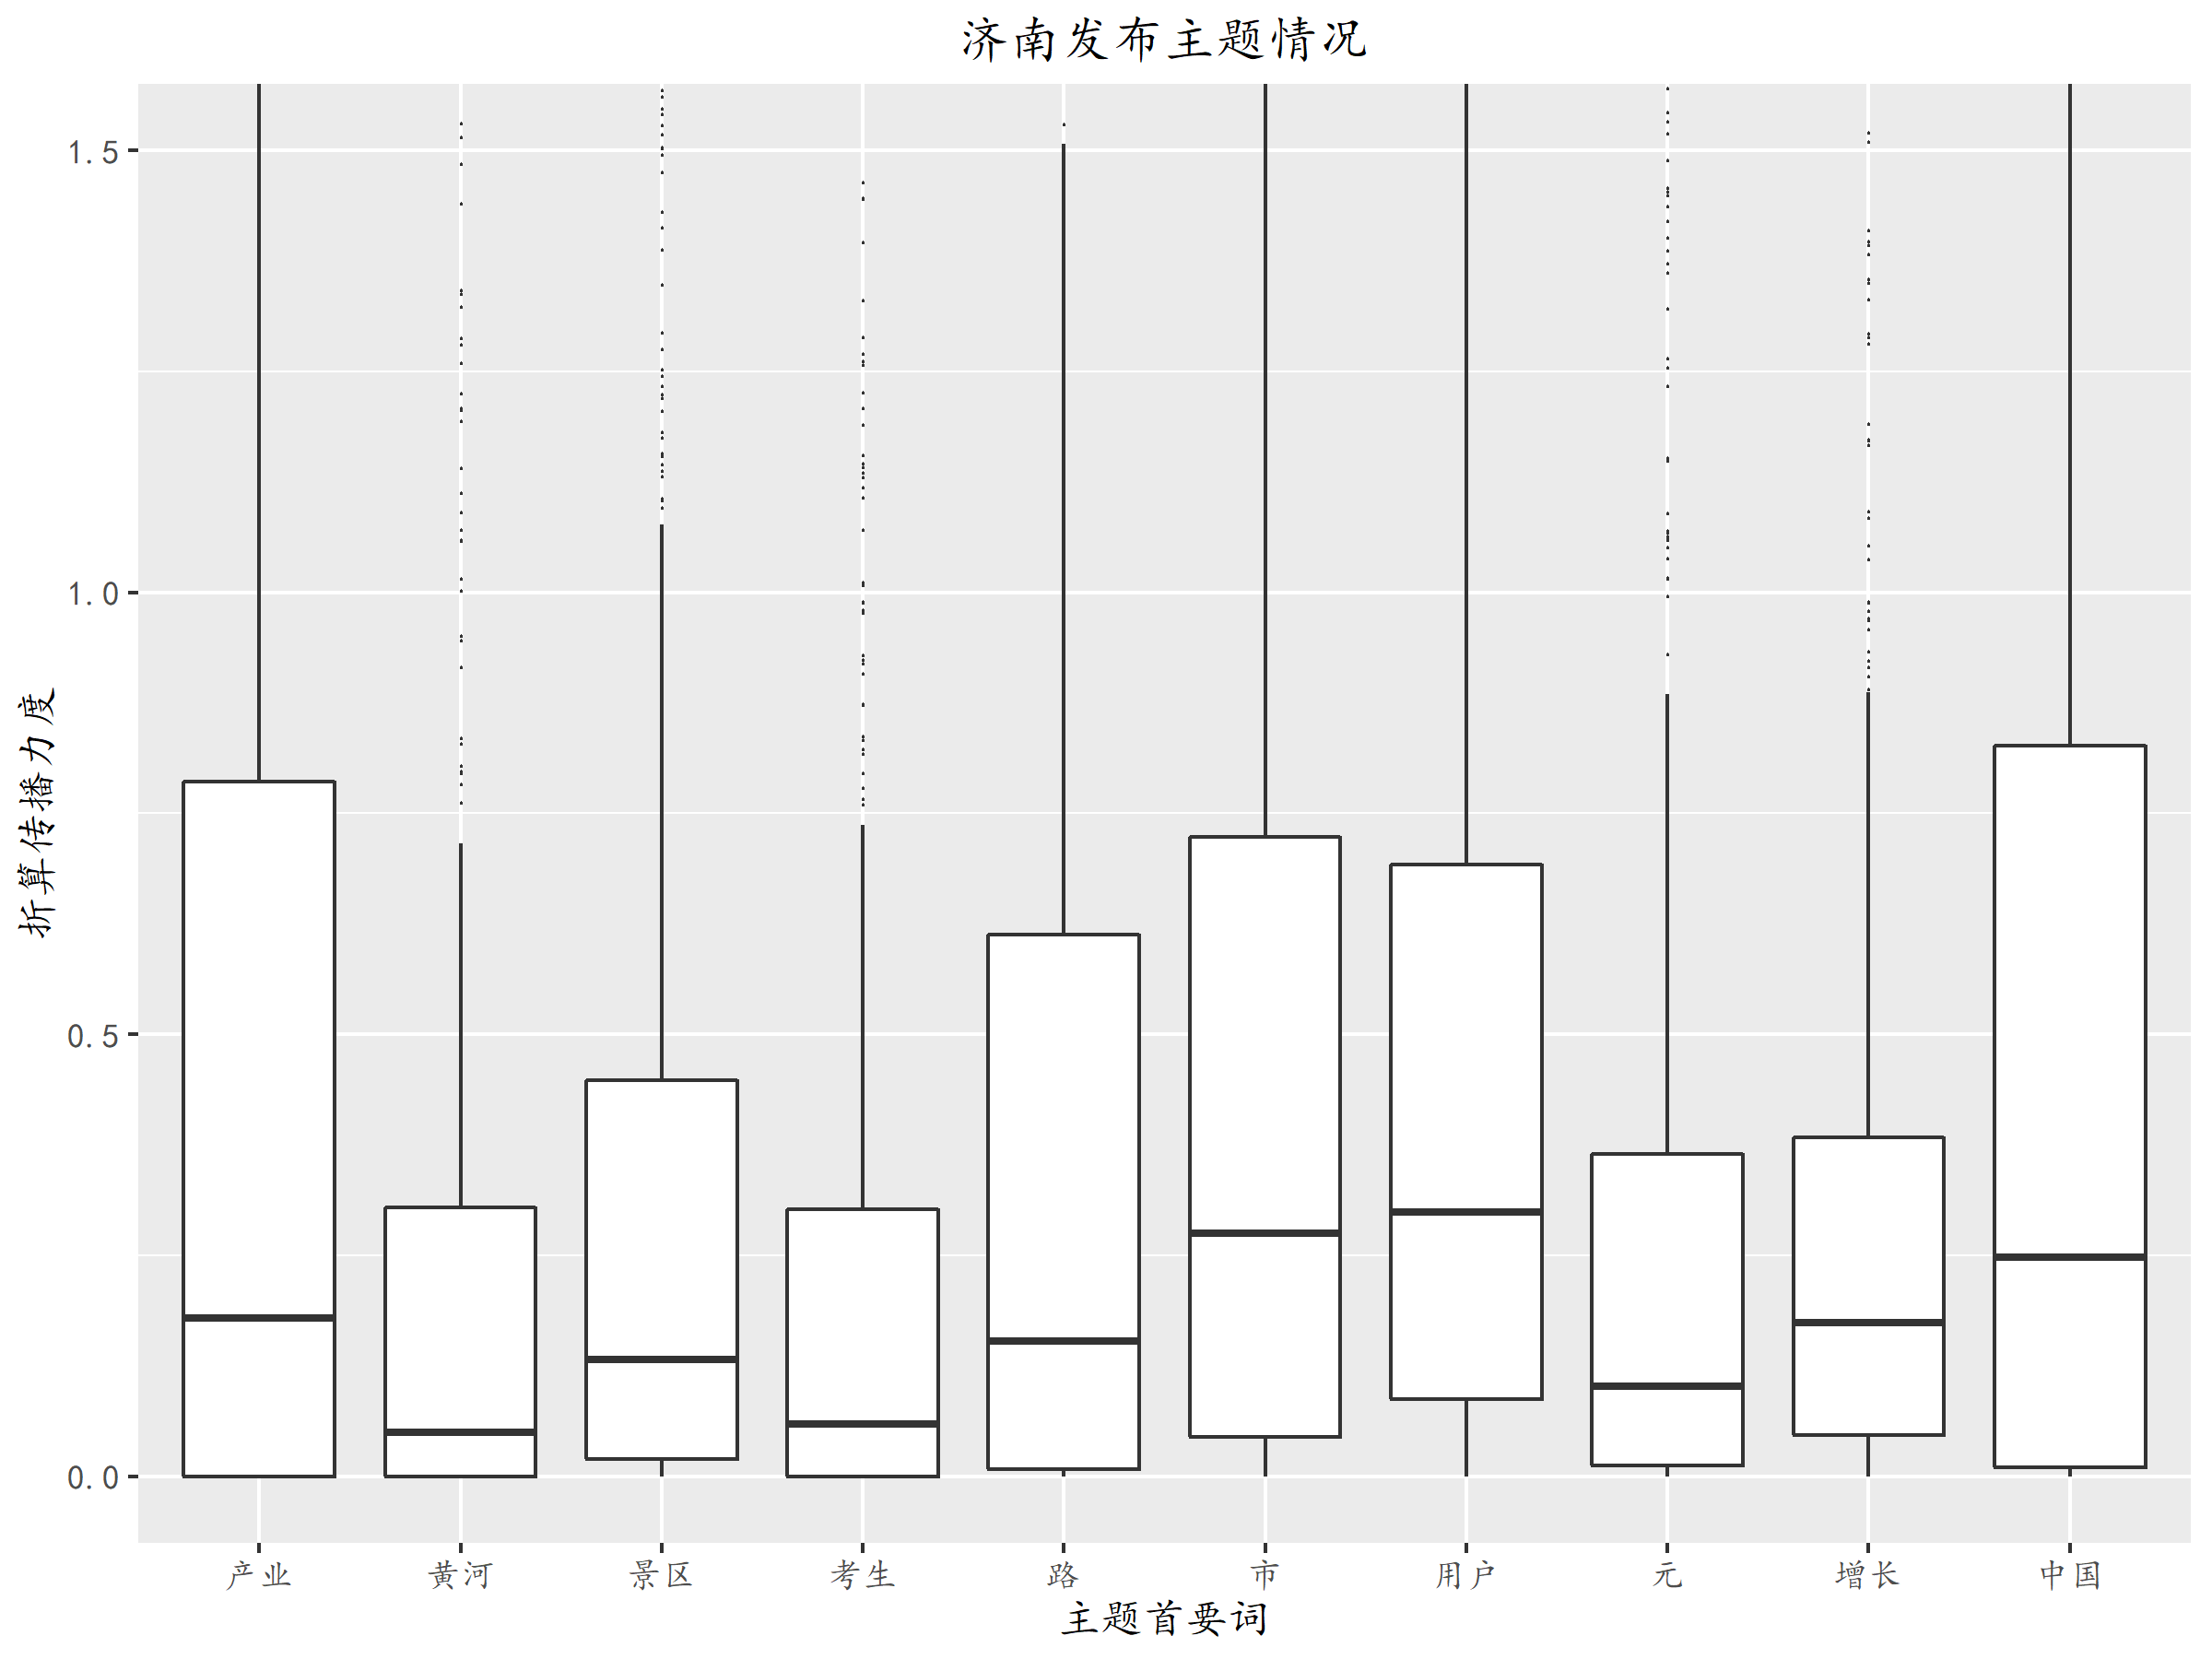
\includegraphics[width=0.9\linewidth]{济南发布.png}
  \caption{"济南发布"公众号各主题下推送传播效力分布}
  \label{fig:济南发布-box}
\end{figure}

\begin{figure}
  \centering
  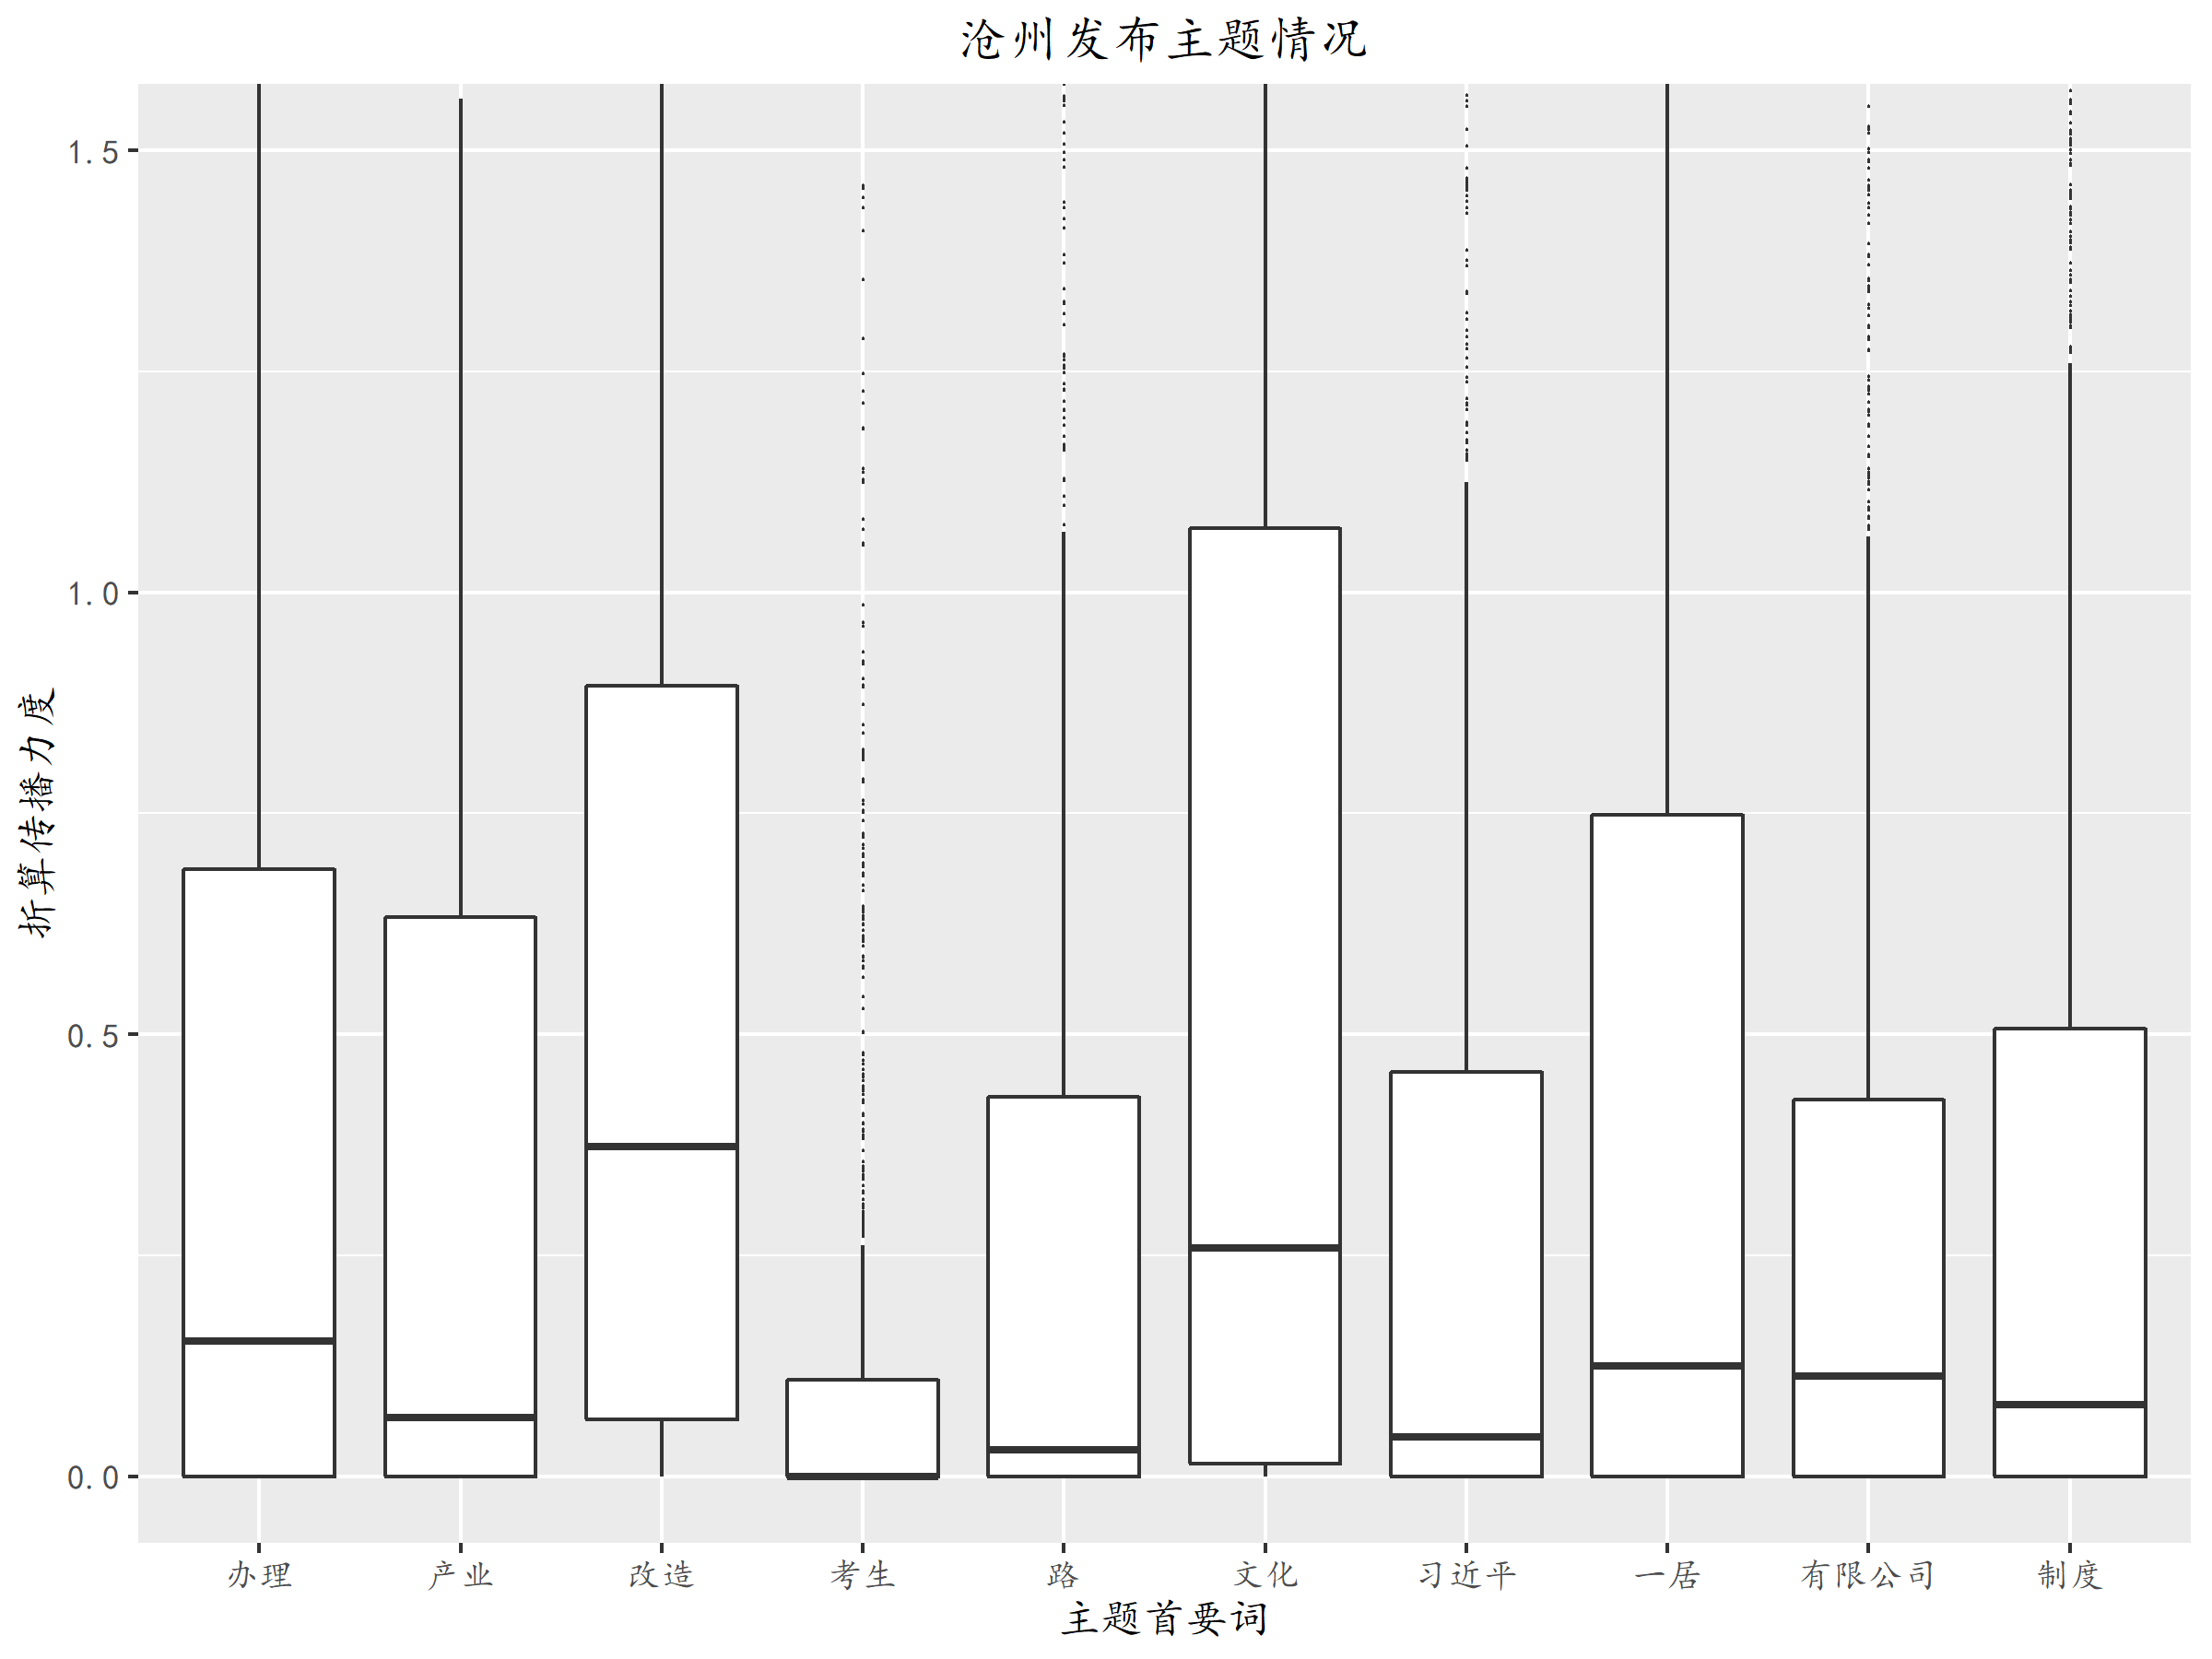
\includegraphics[width=0.9\linewidth]{沧州发布.png}
  \caption{"沧州发布"公众号各主题下推送传播效力分布}
  \label{fig:沧州发布-box}
\end{figure}

\begin{figure}
  \centering
  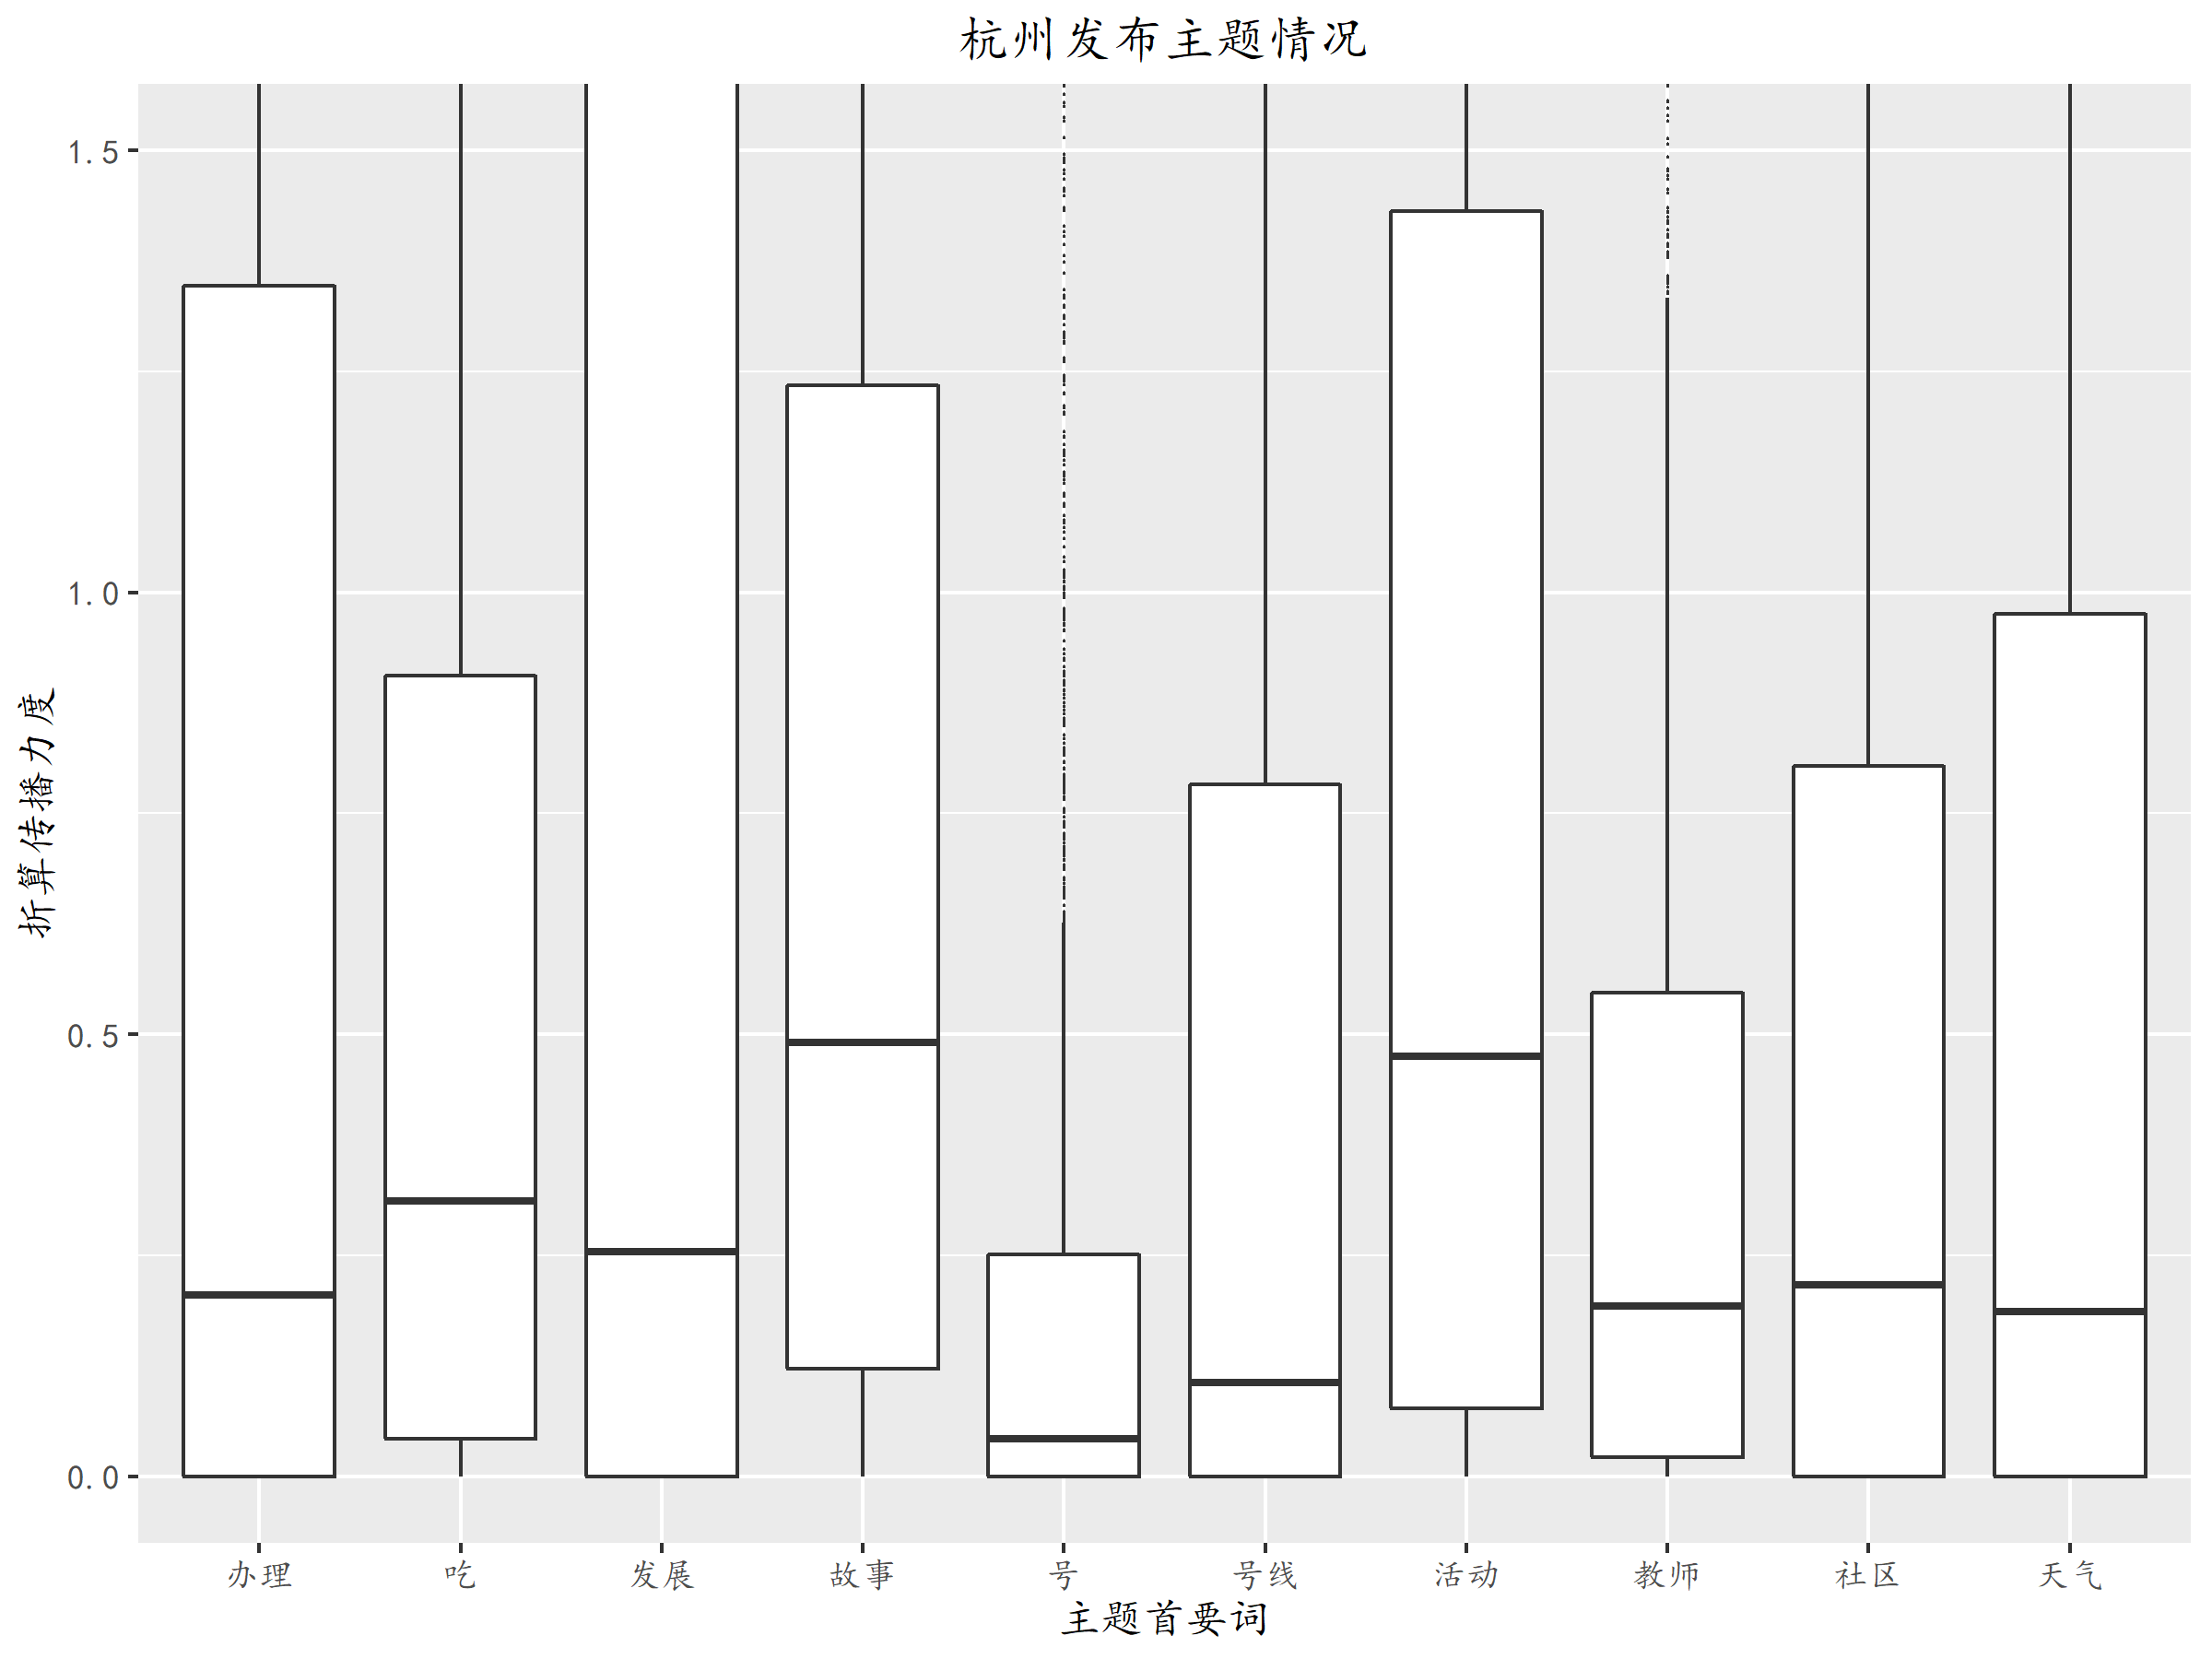
\includegraphics[width=0.9\linewidth]{杭州发布.png}
  \caption{"杭州发布"公众号各主题下推送传播效力分布}
  \label{fig:杭州发布-box}
\end{figure}

\begin{figure}
  \centering
  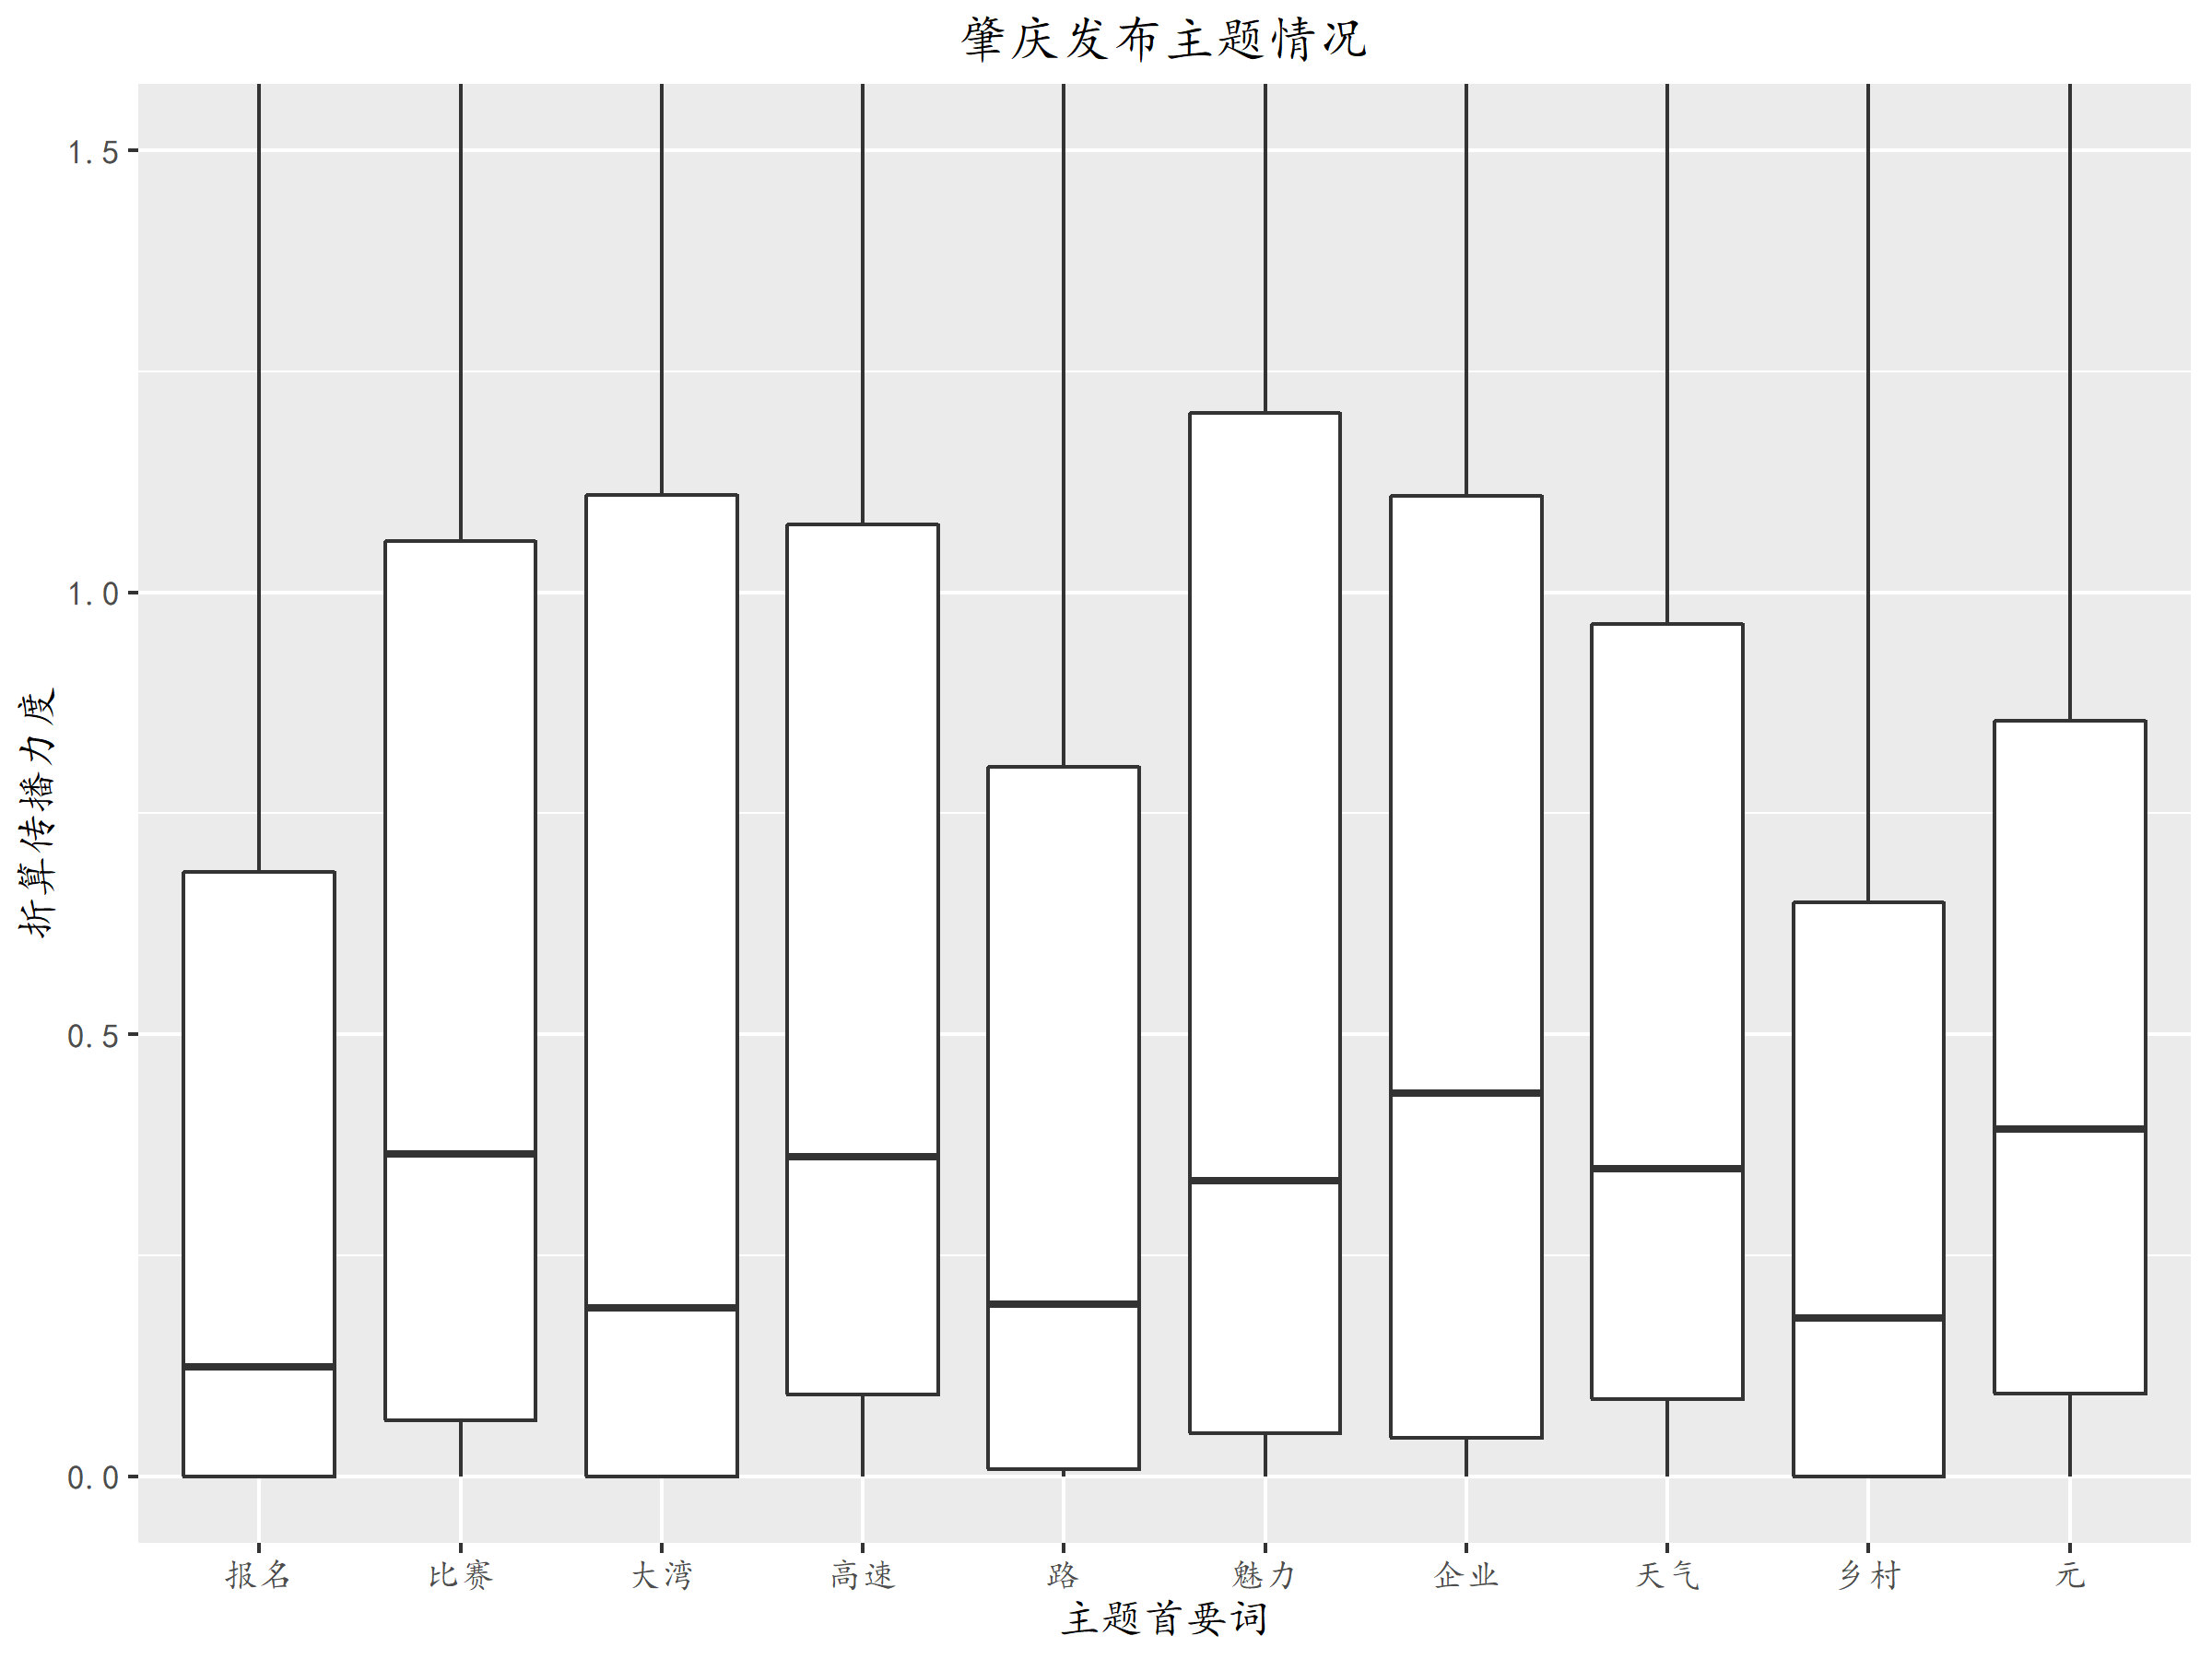
\includegraphics[width=0.9\linewidth]{肇庆发布.png}
  \caption{"肇庆发布"公众号各主题下推送传播效力分布}
  \label{fig:肇庆发布-box}
\end{figure}

\begin{figure}
  \centering
  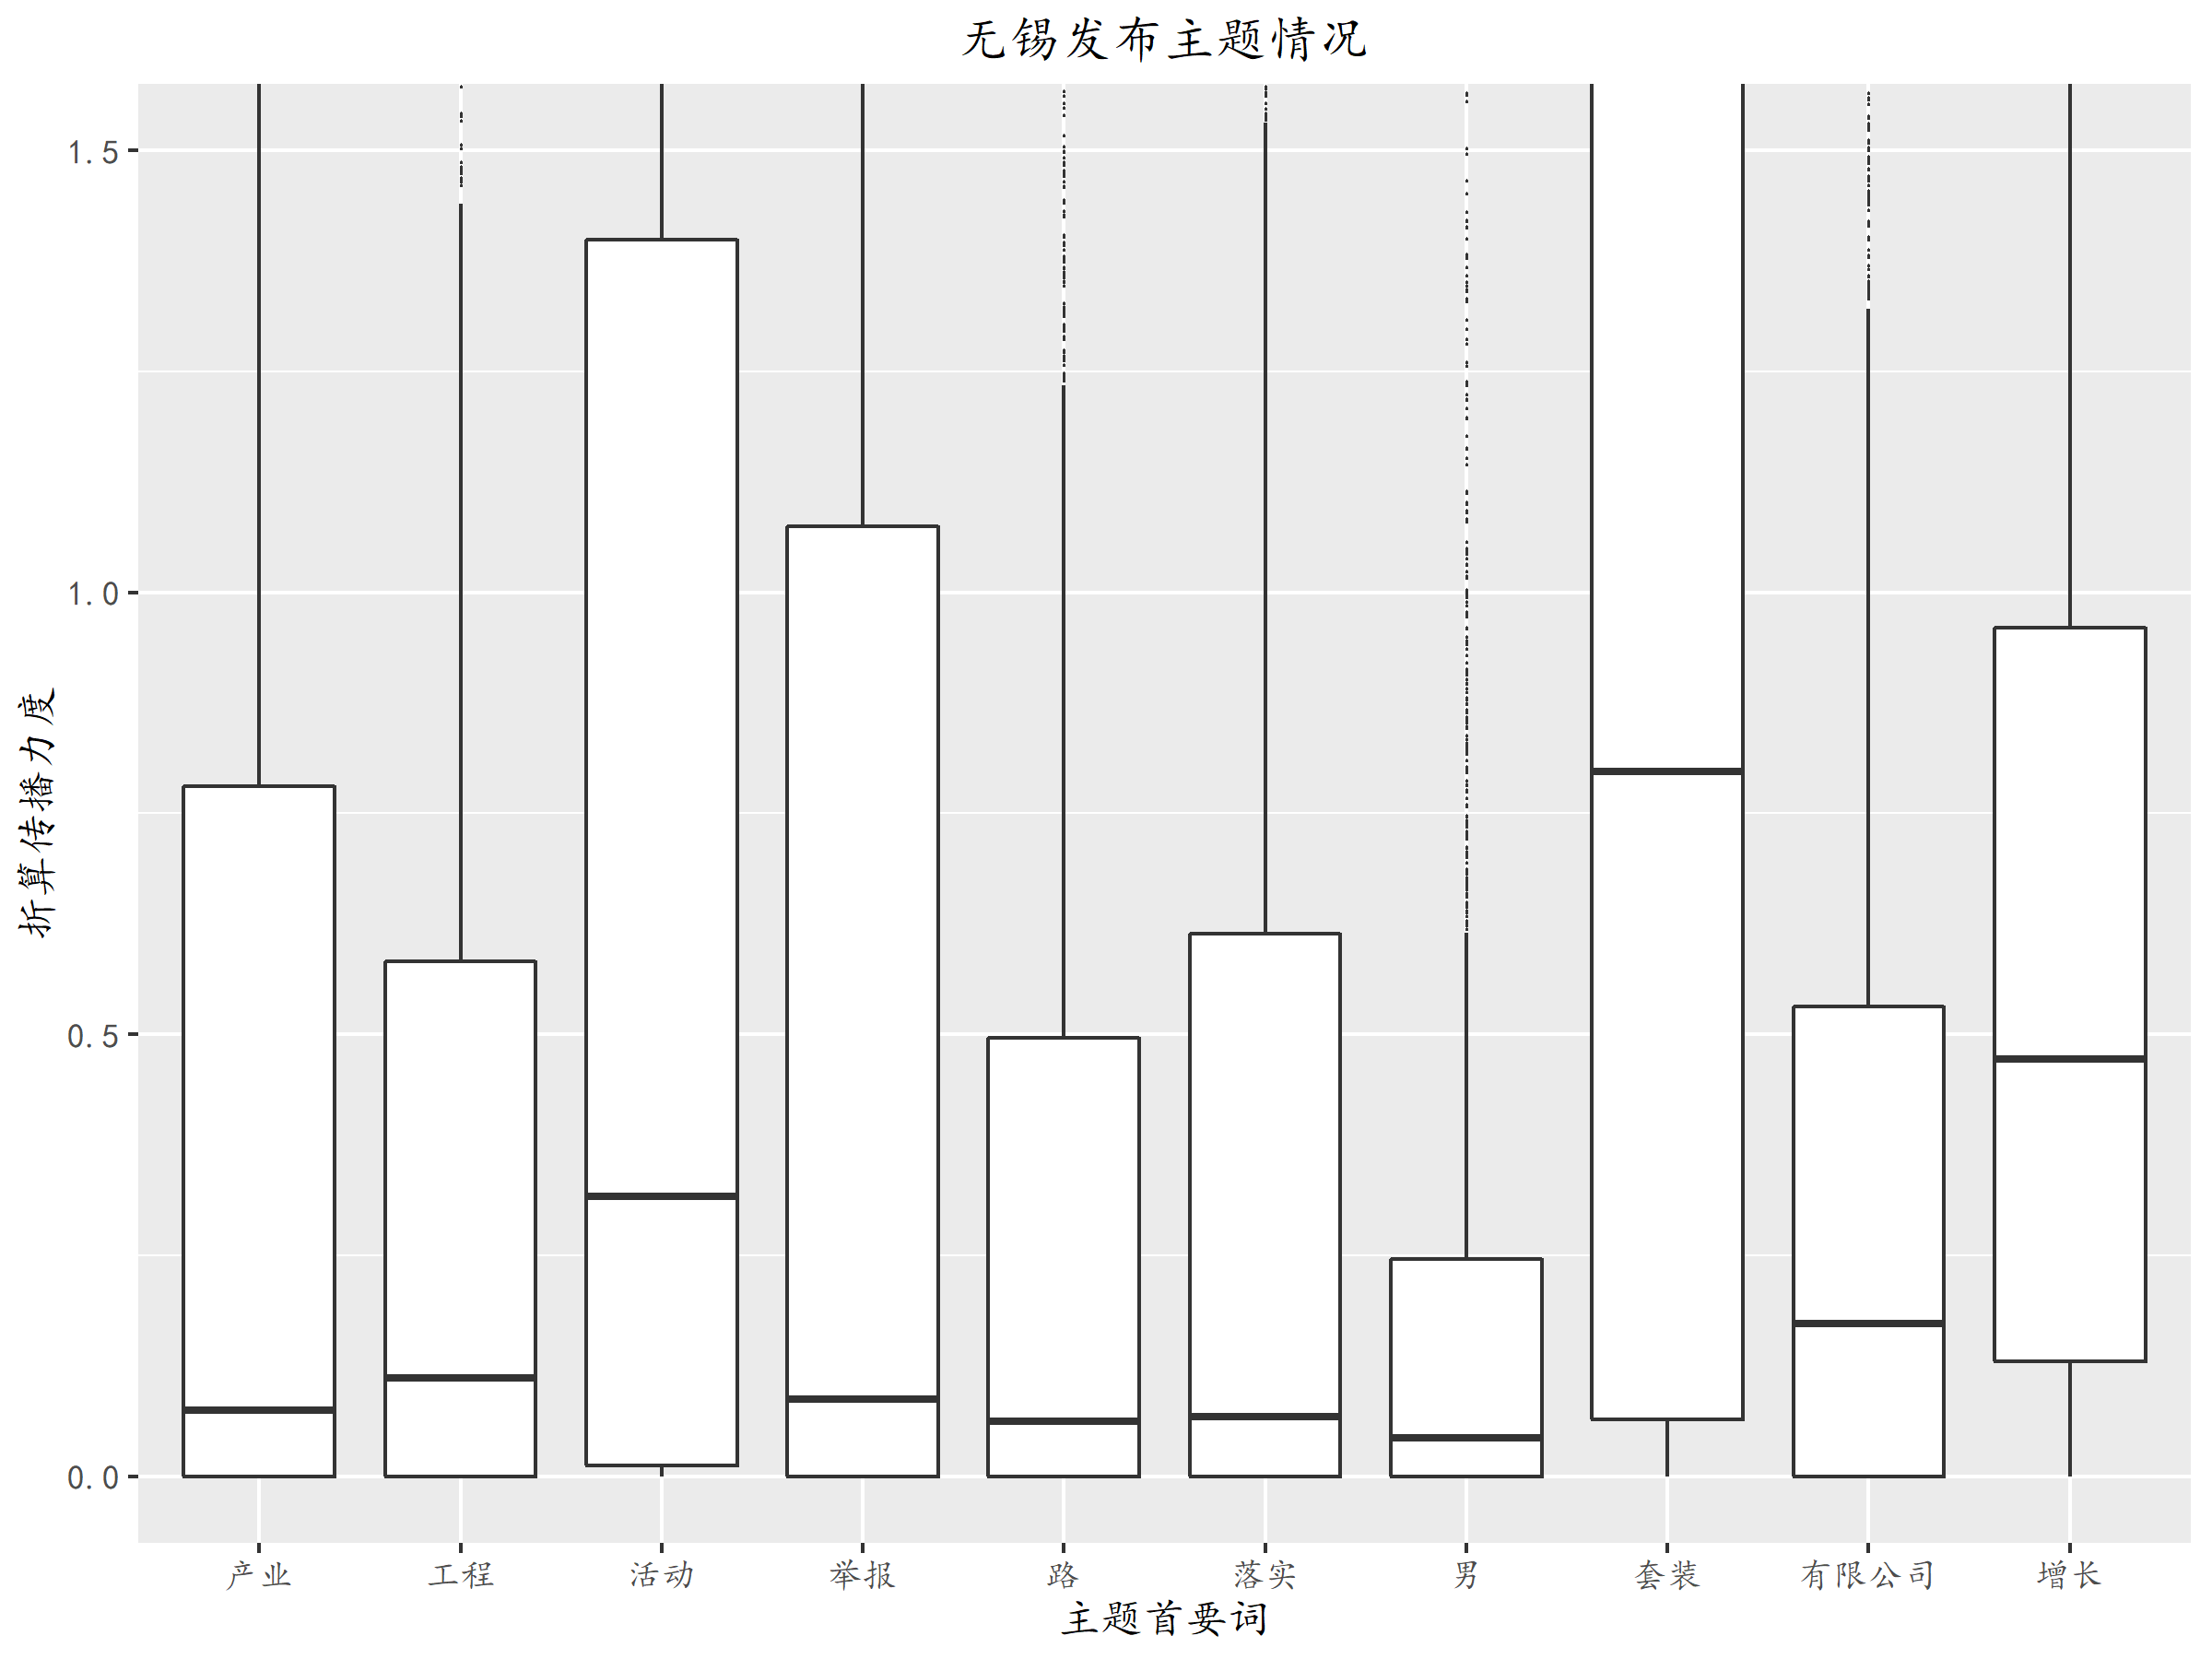
\includegraphics[width=0.9\linewidth]{无锡发布.png}
  \caption{"无锡发布"公众号各主题下推送传播效力分布}
  \label{fig:无锡发布-box}
\end{figure}

\begin{figure}
  \centering
  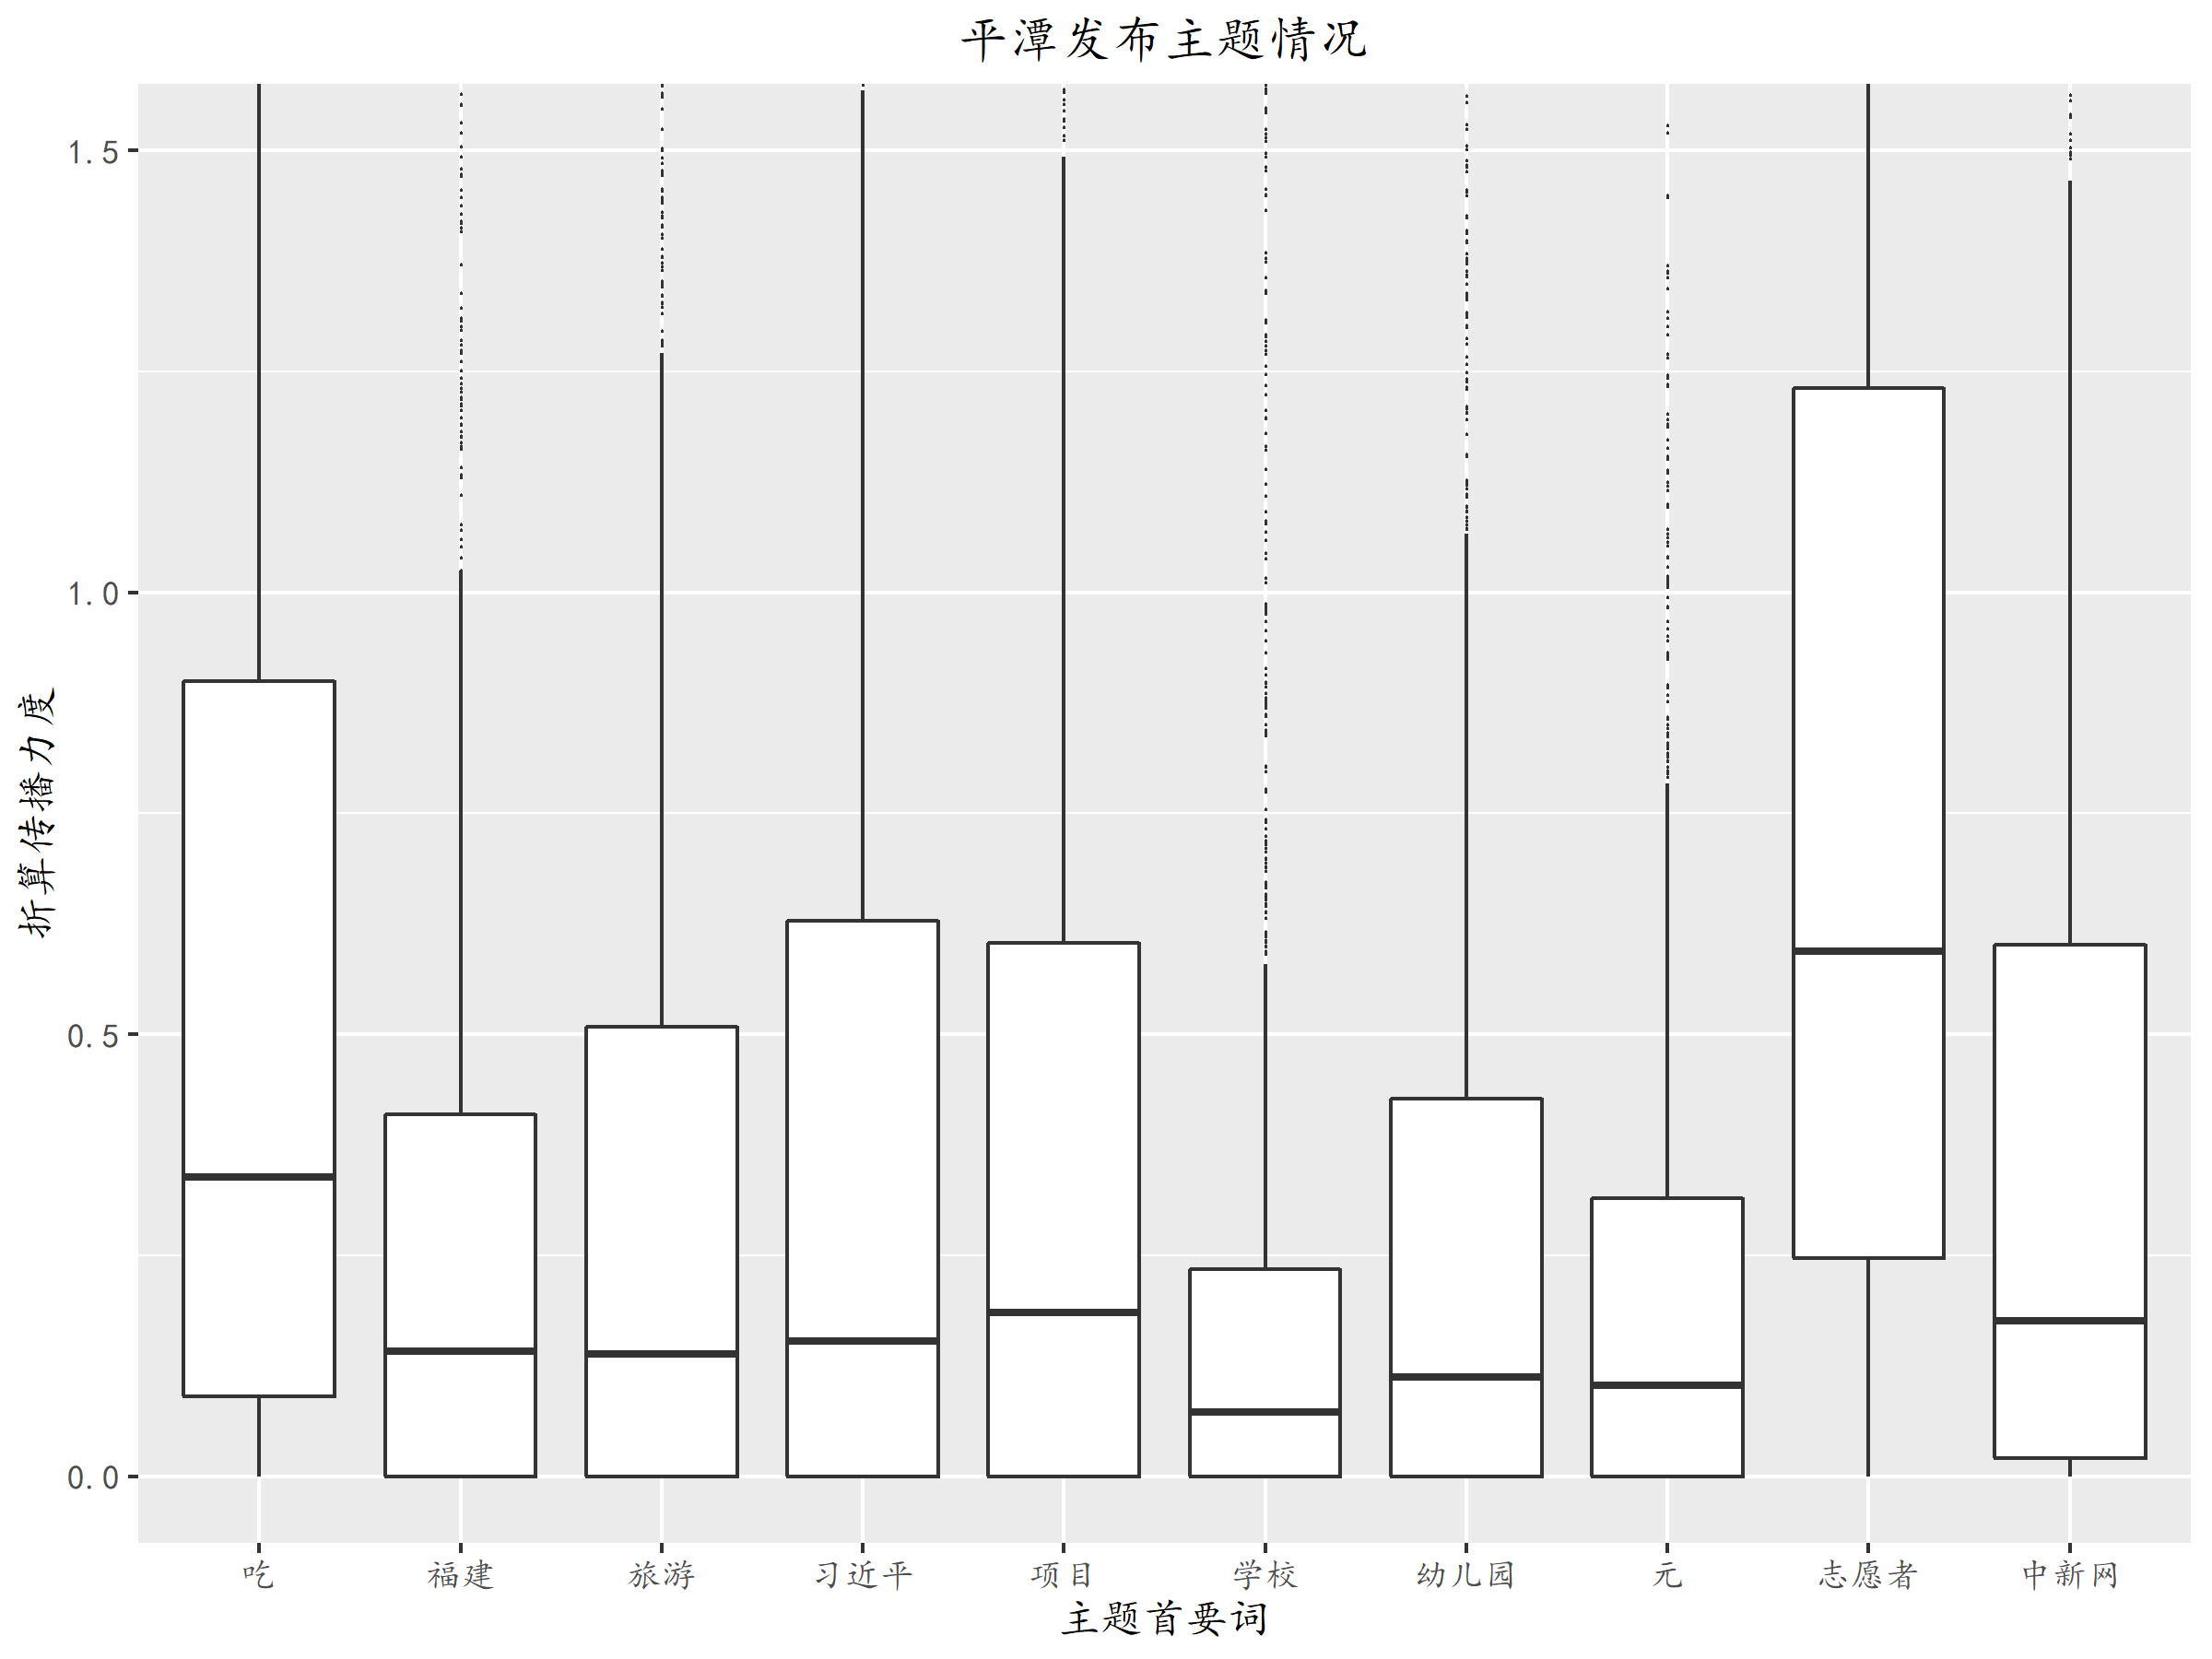
\includegraphics[width=0.9\linewidth]{平潭发布.png}
  \caption{"平潭发布"公众号各主题下推送传播效力分布}
  \label{fig:平潭发布-box}
\end{figure}

\begin{figure}
  \centering
  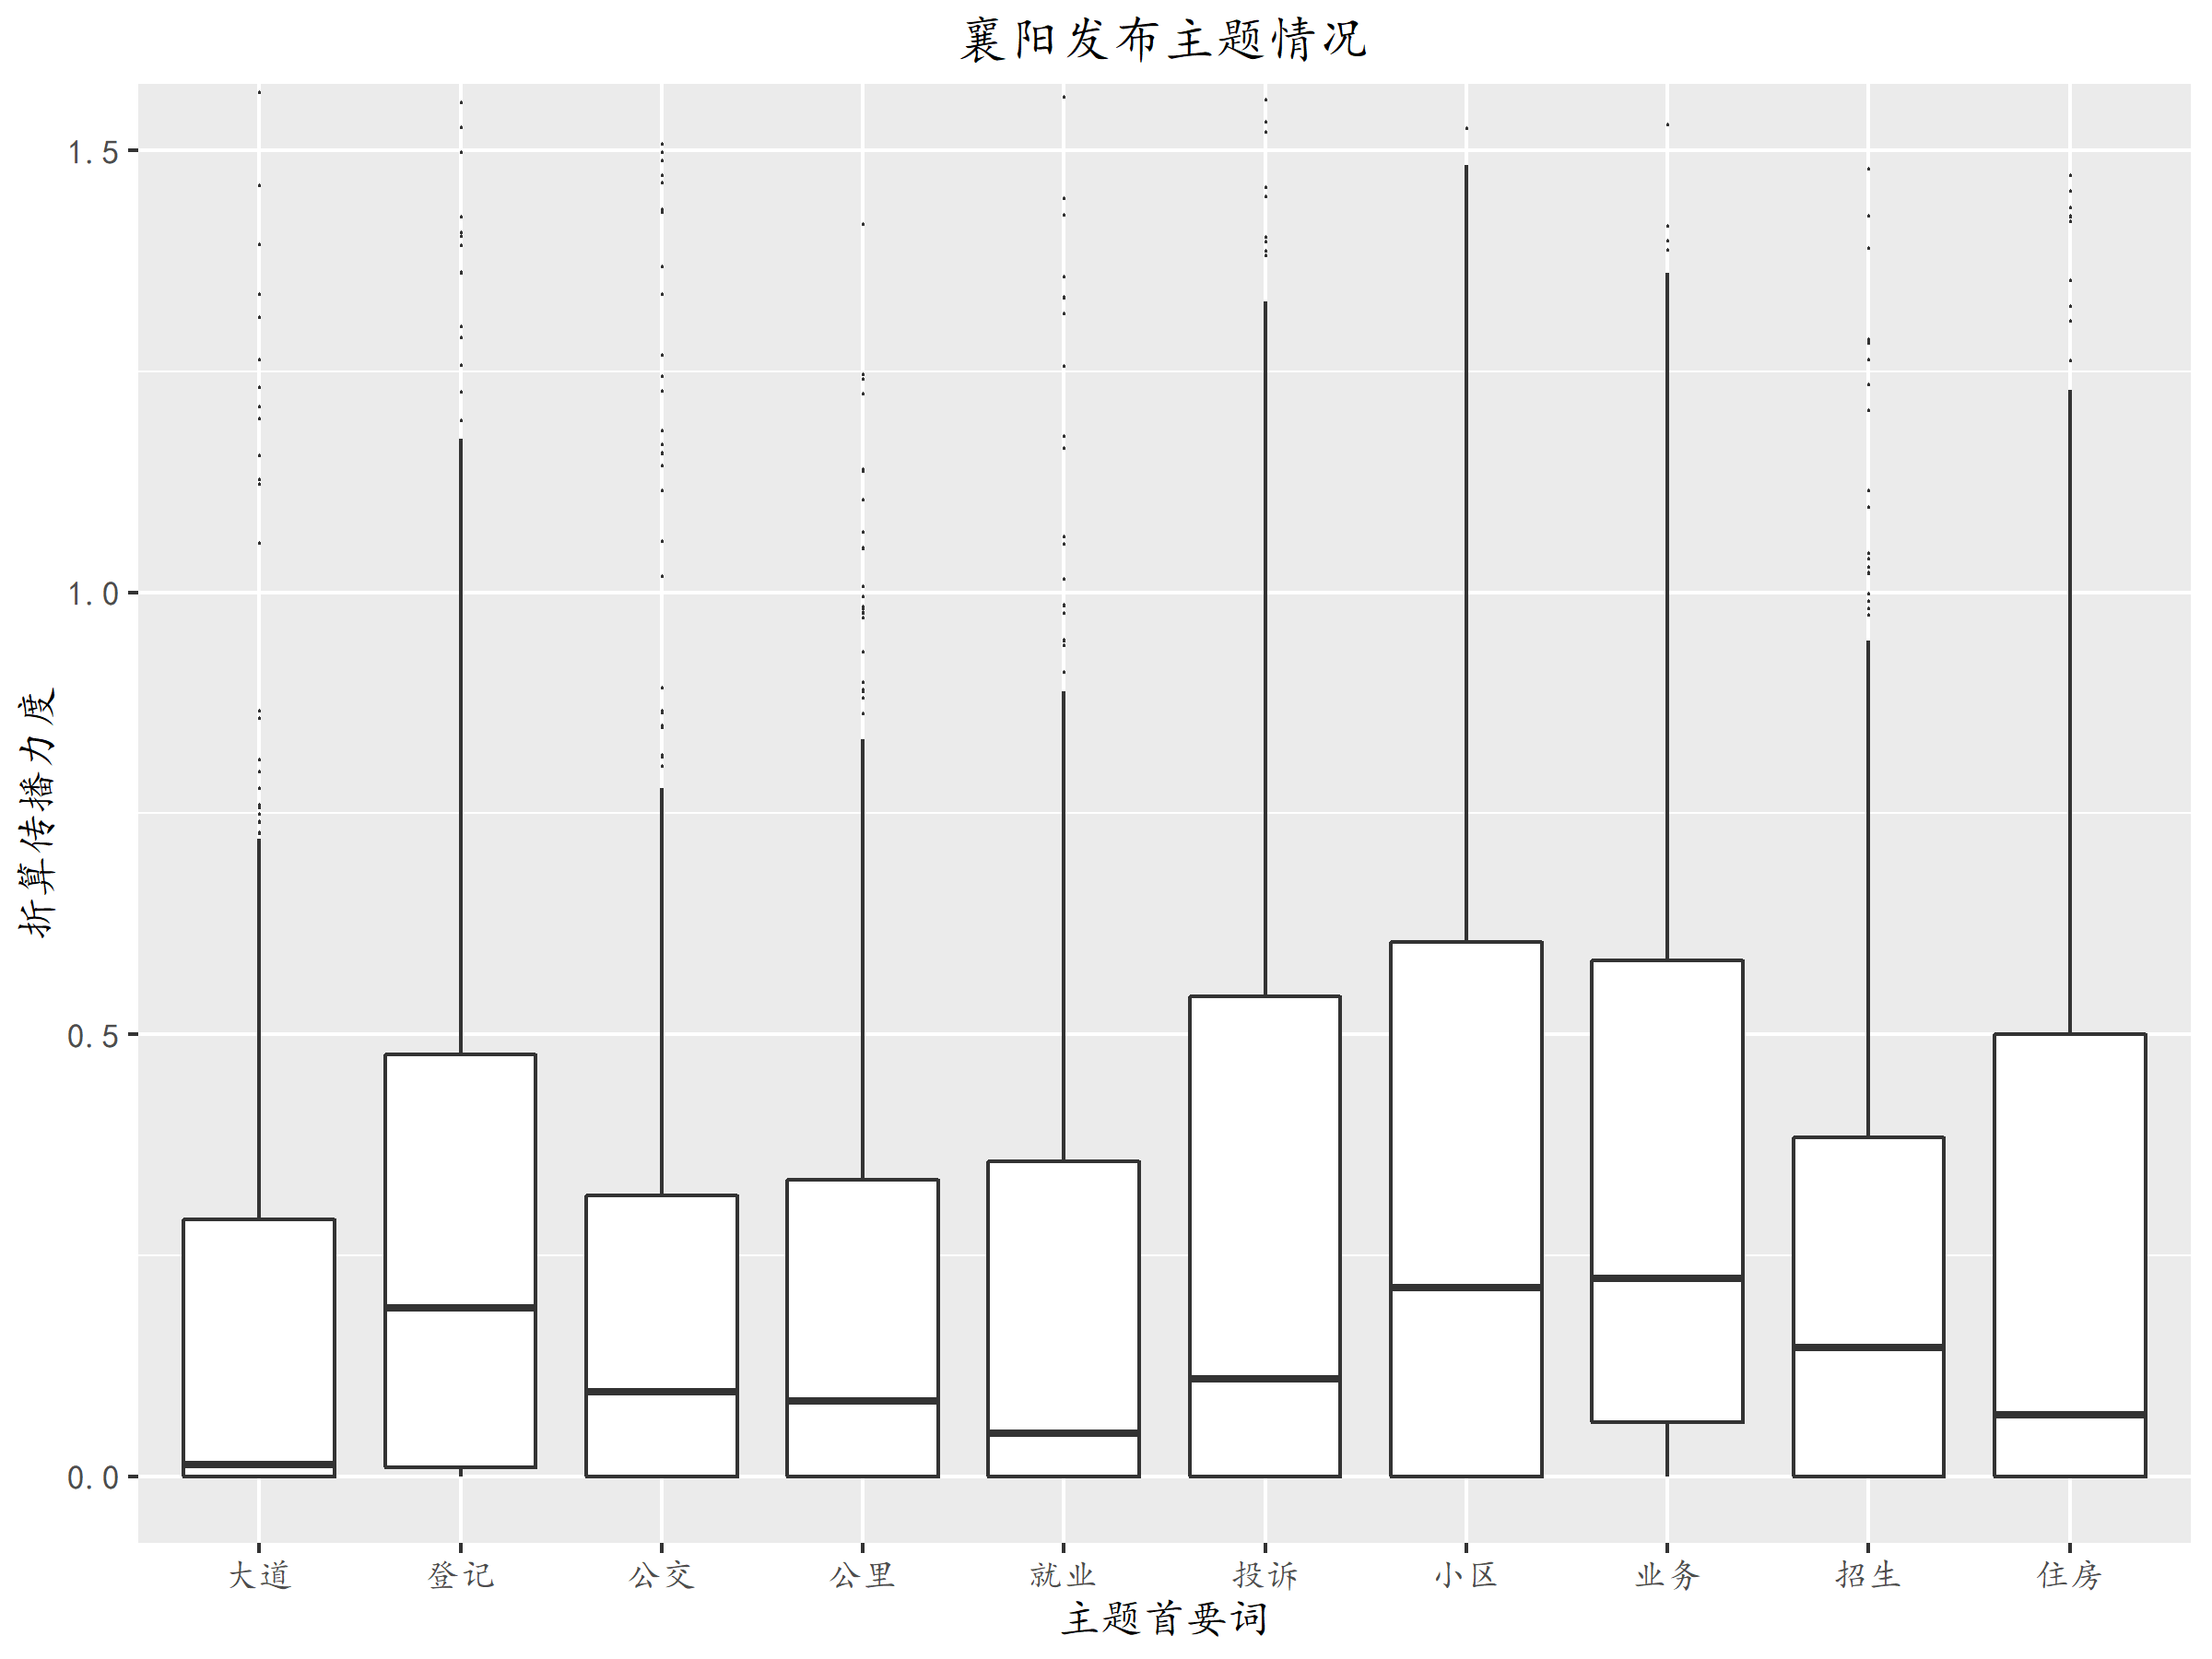
\includegraphics[width=0.9\linewidth]{襄阳发布.png}
  \caption{"襄阳发布"公众号各主题下推送传播效力分布}
  \label{fig:襄阳发布-box}
\end{figure}

\begin{figure}
  \centering
  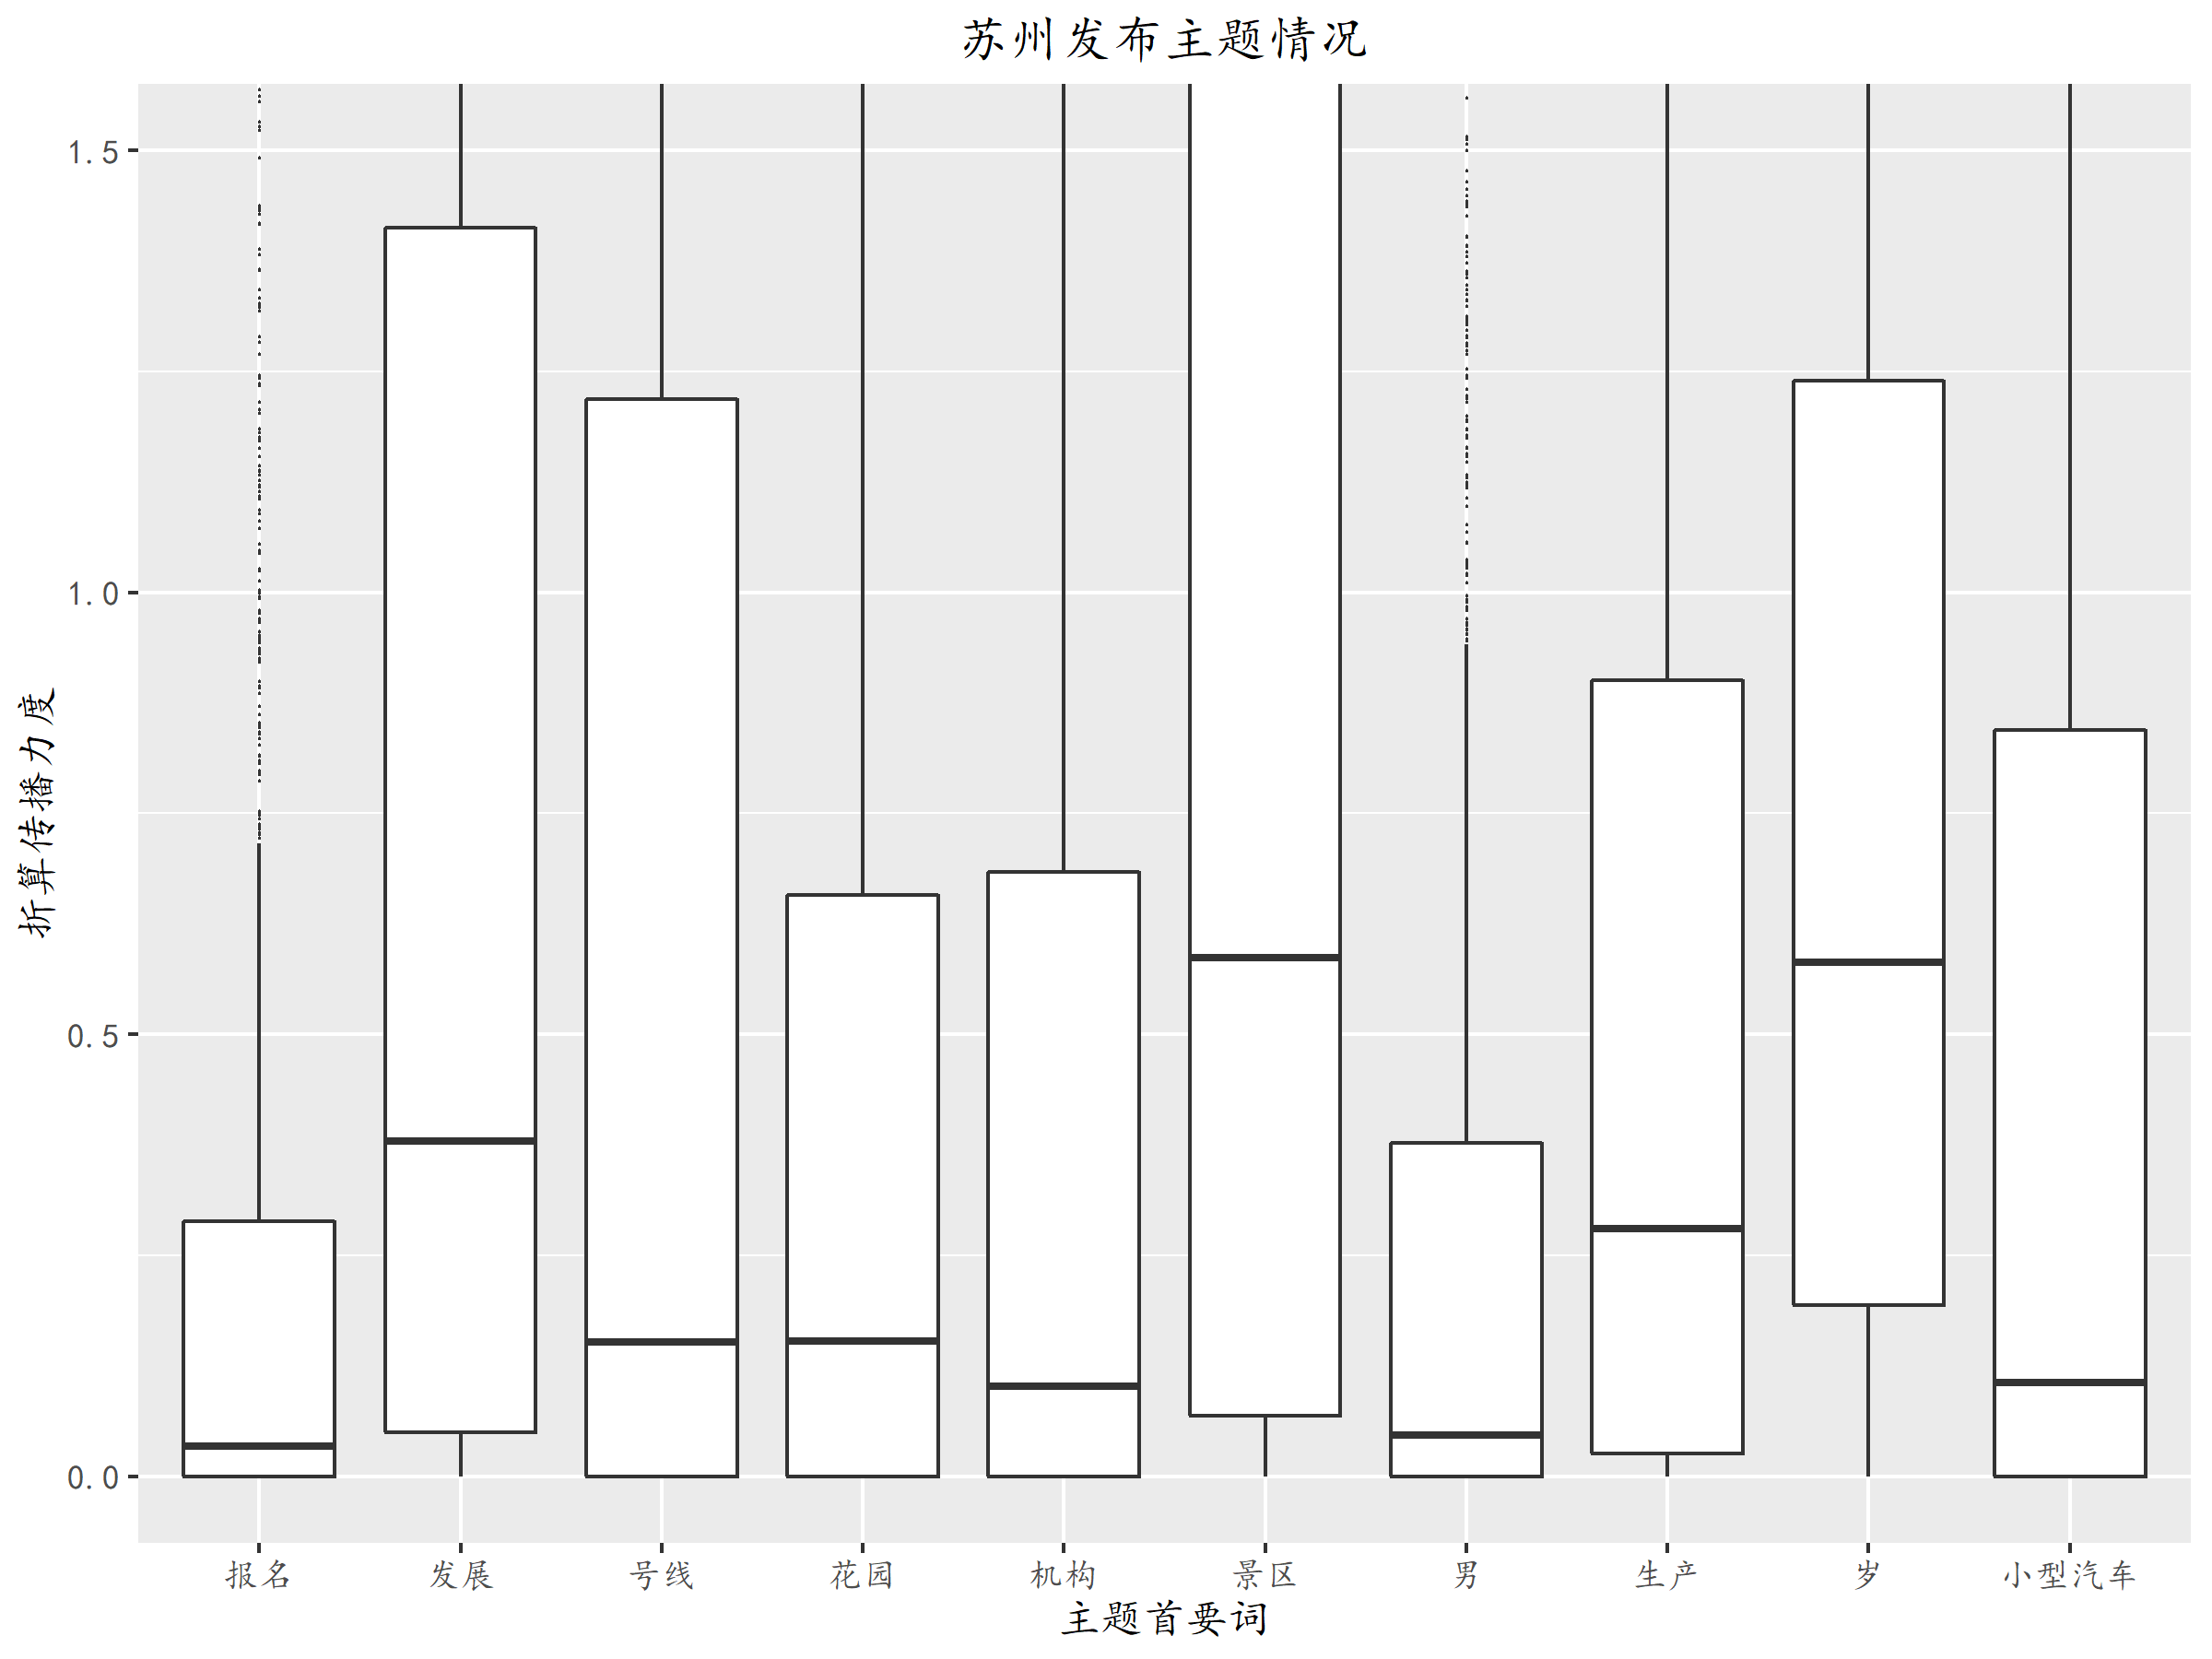
\includegraphics[width=0.9\linewidth]{苏州发布.png}
  \caption{"苏州发布"公众号各主题下推送传播效力分布}
  \label{fig:苏州发布-box}
\end{figure}

\begin{figure}
  \centering
  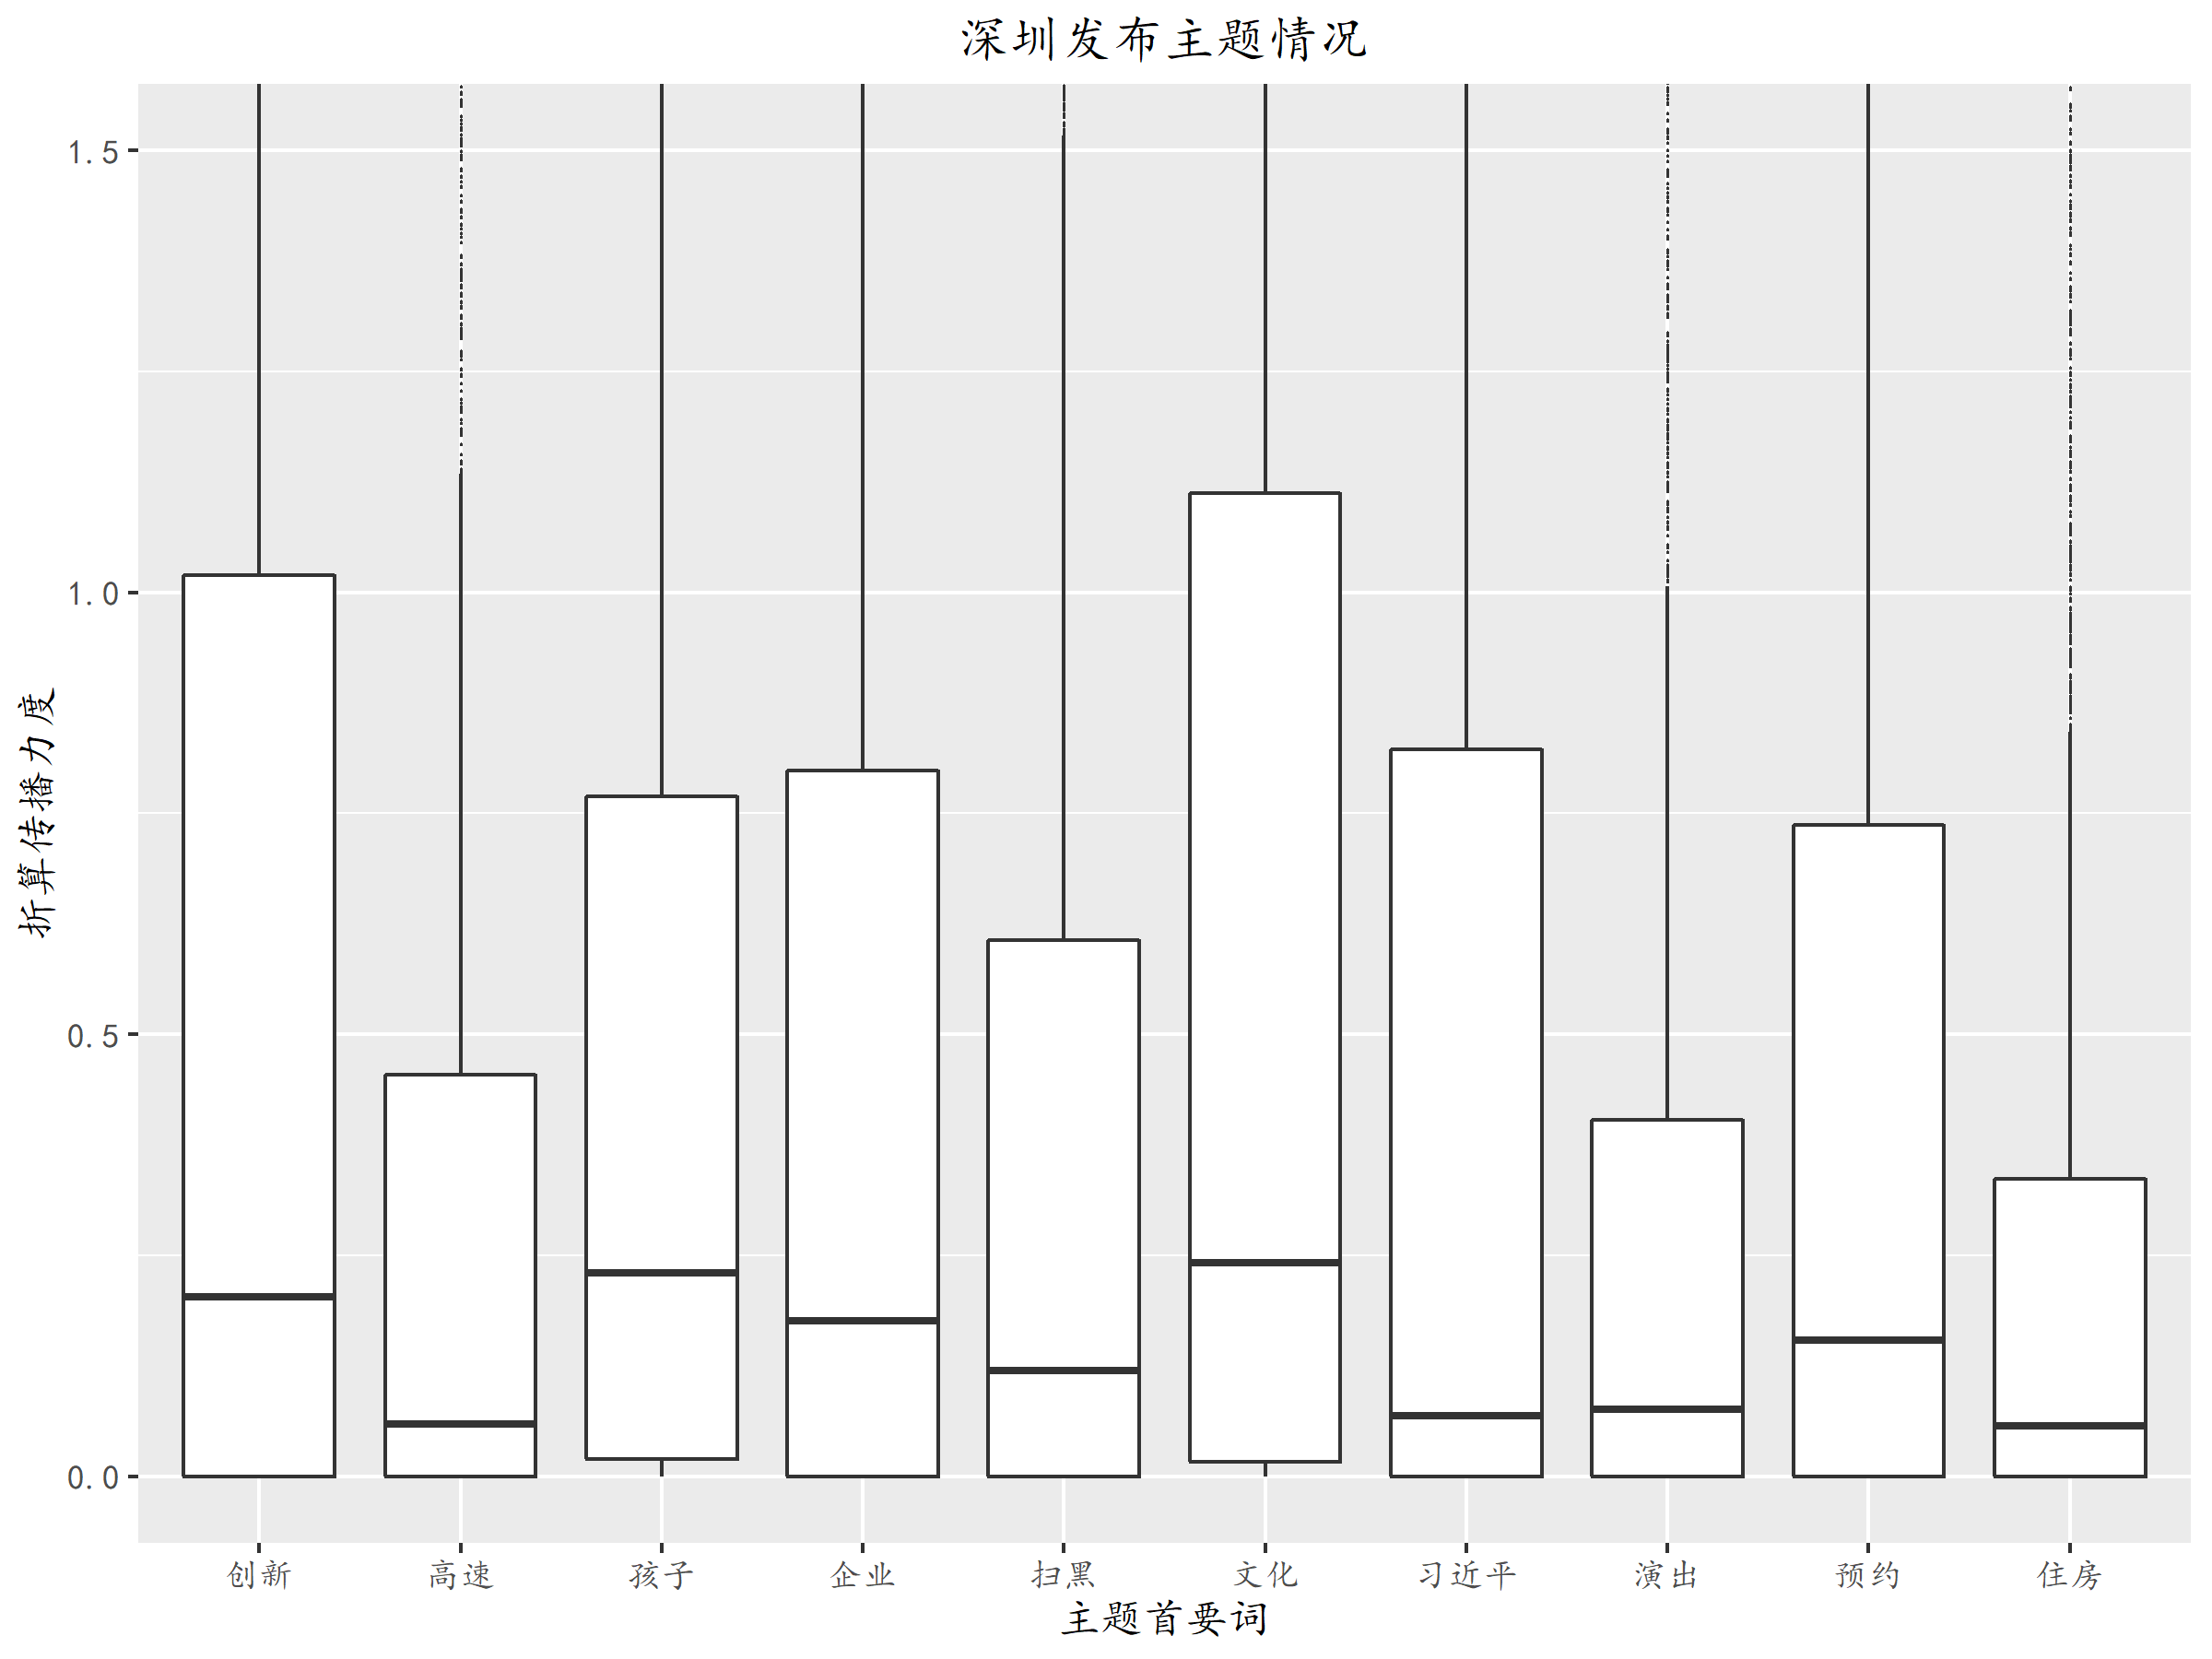
\includegraphics[width=0.9\linewidth]{深圳发布.png}
  \caption{"深圳发布"公众号各主题下推送传播效力分布}
  \label{fig:深圳发布-box}
\end{figure}

    \subsection{官媒主题效力分析}
    
    \label{applastpage}
    \newpage
    \bibliography{report}
    \bibliographystyle{unsrt}
\iffalse
\begin{itemize}[noitemsep,topsep=0pt]
%no white space
\end{itemize}
\begin{enumerate}[label=\Roman{*}.,noitemsep,topsep=0pt]
%use upper case roman
\end{enumerate}
\begin{multicols}{2}
%two columns
\end{multicols}
\begin{figure}
  \centering
  \includegraphics[width=0.9\linewidth]{}
  \caption{}
  \label{fig:}
\end{figure}
\fi
\end{document}
